% This file was converted to LaTeX by Writer2LaTeX ver. 0.5
% see http://www.hj-gym.dk/~hj/writer2latex for more info
\documentclass{article}
\usepackage[ascii]{inputenc}
\usepackage[T1]{fontenc}
\usepackage[spanish,english]{babel}
\usepackage{amsmath,amssymb,amsfonts,textcomp}
\usepackage{color}
\usepackage{array}
\usepackage{supertabular}
\usepackage{hhline}
\usepackage{hyperref}
\hypersetup{pdftex, colorlinks=true, linkcolor=blue, citecolor=blue, filecolor=blue, pagecolor=blue, urlcolor=blue, pdftitle=, pdfauthor=qiangwz, pdfsubject=, pdfkeywords=}
\usepackage[pdftex]{graphicx}
% Text styles
\newcommand\textstyleInternetlink[1]{\textcolor[rgb]{0.0,0.0,0.5019608}{#1}}
% Outline numbering
\setcounter{secnumdepth}{4}
\renewcommand\thesection{\arabic{section}.}
\renewcommand\thesubsection{\arabic{subsection}.}
\renewcommand\thesubsubsection{\arabic{subsection}.\arabic{subsubsection}.}
\renewcommand\theparagraph{\arabic{subsection}.\arabic{subsubsection}.\arabic{paragraph}.}
\makeatletter
\newcommand\arraybslash{\let\\\@arraycr}
\makeatother
% List styles
\newcommand\liststyleWWviiiNumii{%
\renewcommand\labelitemi{[F0B7?]}
\renewcommand\labelitemii{[F0B7?]}
\renewcommand\labelitemiii{[F0B7?]}
\renewcommand\labelitemiv{[F0B7?]}
}
\newcommand\liststyleWWviiiNumxiii{%
\renewcommand\labelitemi{[F0B7?]}
\renewcommand\labelitemii{[F0B7?]}
\renewcommand\labelitemiii{[F0B7?]}
\renewcommand\labelitemiv{[F0B7?]}
}
\newcommand\liststyleWWviiiNumxxi{%
\renewcommand\labelitemi{[F0B7?]}
\renewcommand\labelitemii{o}
\renewcommand\labelitemiii{[F0A7?]}
\renewcommand\labelitemiv{[F0B7?]}
}
\newcommand\liststyleWWviiiNumxvii{%
\renewcommand\labelitemi{o}
\renewcommand\labelitemii{o}
\renewcommand\labelitemiii{[F0A7?]}
\renewcommand\labelitemiv{[F0B7?]}
}
\newcommand\liststyleWWviiiNumxix{%
\renewcommand\theenumi{\arabic{enumi}}
\renewcommand\theenumii{\arabic{enumii}}
\renewcommand\theenumiii{\arabic{enumiii}}
\renewcommand\labelitemi{o}
\renewcommand\labelenumi{\theenumi.}
\renewcommand\labelenumii{\theenumii.}
\renewcommand\labelenumiii{\theenumiii.}
}
\newcommand\liststyleWWviiiNumxviii{%
\renewcommand\labelitemi{o}
\renewcommand\labelitemii{o}
\renewcommand\labelitemiii{[F0A7?]}
\renewcommand\labelitemiv{[F0B7?]}
}
\newcommand\liststyleWWviiiNumxx{%
\renewcommand\theenumi{\arabic{enumi}}
\renewcommand\theenumii{\arabic{enumii}}
\renewcommand\theenumiii{\arabic{enumiii}}
\renewcommand\labelitemi{o}
\renewcommand\labelenumi{\theenumi.}
\renewcommand\labelenumii{\theenumii.}
\renewcommand\labelenumiii{\theenumiii.}
}
\newcommand\liststyleWWviiiNumxxii{%
\renewcommand\theenumi{\arabic{enumi}}
\renewcommand\theenumii{\arabic{enumii}}
\renewcommand\theenumiii{\arabic{enumiii}}
\renewcommand\labelitemi{o}
\renewcommand\labelenumi{\theenumi.}
\renewcommand\labelenumii{\theenumii.}
\renewcommand\labelenumiii{\theenumiii.}
}
\newcommand\liststyleWWviiiNumxxiii{%
\renewcommand\theenumi{\arabic{enumi}}
\renewcommand\theenumii{\arabic{enumii}}
\renewcommand\theenumiii{\arabic{enumiii}}
\renewcommand\labelitemi{{}-}
\renewcommand\labelenumi{\theenumi.}
\renewcommand\labelenumii{\theenumii.}
\renewcommand\labelenumiii{\theenumiii.}
}
\newcommand\liststyleWWviiiNumiii{%
\renewcommand\theenumi{\alph{enumi}}
\renewcommand\theenumii{\arabic{enumii}}
\renewcommand\theenumiii{\arabic{enumiii}}
\renewcommand\theenumiv{\arabic{enumiv}}
\renewcommand\labelenumi{\theenumi)}
\renewcommand\labelenumii{\theenumii.}
\renewcommand\labelenumiii{\theenumiii.}
\renewcommand\labelenumiv{\theenumiv.}
}
\newcommand\liststyleWWviiiNumiv{%
\renewcommand\theenumi{\alph{enumi}}
\renewcommand\theenumii{\arabic{enumii}}
\renewcommand\theenumiii{\arabic{enumiii}}
\renewcommand\theenumiv{\arabic{enumiv}}
\renewcommand\labelenumi{\theenumi)}
\renewcommand\labelenumii{\theenumii.}
\renewcommand\labelenumiii{\theenumiii.}
\renewcommand\labelenumiv{\theenumiv.}
}
\newcommand\liststyleWWviiiNumv{%
\renewcommand\theenumi{\alph{enumi}}
\renewcommand\theenumii{\arabic{enumii}}
\renewcommand\theenumiii{\arabic{enumiii}}
\renewcommand\theenumiv{\arabic{enumiv}}
\renewcommand\labelenumi{\theenumi)}
\renewcommand\labelenumii{\theenumii.}
\renewcommand\labelenumiii{\theenumiii.}
\renewcommand\labelenumiv{\theenumiv.}
}
\newcommand\liststyleWWviiiNumvi{%
\renewcommand\theenumi{\alph{enumi}}
\renewcommand\theenumii{\arabic{enumii}}
\renewcommand\theenumiii{\arabic{enumiii}}
\renewcommand\theenumiv{\arabic{enumiv}}
\renewcommand\labelenumi{\theenumi)}
\renewcommand\labelenumii{\theenumii.}
\renewcommand\labelenumiii{\theenumiii.}
\renewcommand\labelenumiv{\theenumiv.}
}
\newcommand\liststyleWWviiiNumvii{%
\renewcommand\theenumi{\alph{enumi}}
\renewcommand\theenumii{\arabic{enumii}}
\renewcommand\theenumiii{\arabic{enumiii}}
\renewcommand\theenumiv{\arabic{enumiv}}
\renewcommand\labelenumi{\theenumi)}
\renewcommand\labelenumii{\theenumii.}
\renewcommand\labelenumiii{\theenumiii.}
\renewcommand\labelenumiv{\theenumiv.}
}
\newcommand\liststyleWWviiiNumviii{%
\renewcommand\labelitemi{[F0B7?]}
\renewcommand\labelitemii{[F081?]}
\renewcommand\labelitemiii{${\blacksquare}$}
\renewcommand\labelitemiv{[F06C?]}
}
\newcommand\liststyleWWviiiNumix{%
\renewcommand\labelitemi{[F0B7?]}
\renewcommand\labelitemii{{}-}
\renewcommand\labelitemiii{${\blacksquare}$}
\renewcommand\labelitemiv{[F06C?]}
}
\newcommand\liststyleWWviiiNumx{%
\renewcommand\labelitemi{[F0B7?]}
\renewcommand\labelitemii{[F081?]}
\renewcommand\labelitemiii{${\blacksquare}$}
\renewcommand\labelitemiv{[F06C?]}
}
\newcommand\liststyleWWviiiNumxiv{%
\renewcommand\theenumi{\arabic{enumi}}
\renewcommand\theenumii{\arabic{enumii}}
\renewcommand\theenumiii{\arabic{enumiii}}
\renewcommand\theenumiv{\arabic{enumiv}}
\renewcommand\labelenumi{\theenumi.}
\renewcommand\labelenumii{\theenumii.}
\renewcommand\labelenumiii{\theenumiii.}
\renewcommand\labelenumiv{\theenumiv.}
}
\newcommand\liststyleLi{%
\renewcommand\theenumi{\arabic{enumi}}
\renewcommand\theenumii{\arabic{enumii}}
\renewcommand\theenumiii{\arabic{enumiii}}
\renewcommand\theenumiv{\arabic{enumiv}}
\renewcommand\labelenumi{\theenumi.}
\renewcommand\labelenumii{\theenumii.}
\renewcommand\labelenumiii{\theenumiii.}
\renewcommand\labelenumiv{\theenumiv.}
}
% Page layout (geometry)
\setlength\paperwidth{8.2673in}
\setlength\paperheight{11.6925in}
\setlength\voffset{-1in}
\setlength\hoffset{-1in}
\setlength\topmargin{1in}
\setlength\oddsidemargin{1.25in}
\setlength\textheight{9.0315in}
\setlength\textwidth{5.7672997in}
\setlength\footskip{0.661in}
\setlength\headheight{0cm}
\setlength\headsep{0cm}
% Footnote rule
\setlength{\skip\footins}{0.0469in}
\renewcommand\footnoterule{\vspace*{-0.0071in}\setlength\leftskip{0pt}\setlength\rightskip{0pt plus 1fil}\noindent\textcolor{black}{\rule{0.25\columnwidth}{0.0071in}}\vspace*{0.0398in}}
% Pages styles
\makeatletter
\newcommand\ps@Convertv{
  \renewcommand\@oddhead{}
  \renewcommand\@evenhead{}
  \renewcommand\@oddfoot{}
  \renewcommand\@evenfoot{\@oddfoot}
  \renewcommand\thepage{\arabic{page}}
}
\newcommand\ps@Standard{
  \renewcommand\@oddhead{}
  \renewcommand\@evenhead{}
  \renewcommand\@oddfoot{\thepage{}}
  \renewcommand\@evenfoot{\@oddfoot}
  \renewcommand\thepage{\arabic{page}}
}
\makeatother
\pagestyle{Standard}
\setlength\tabcolsep{1mm}
\renewcommand\arraystretch{1.3}
\newcounter{Bibitem}
\renewcommand\theBibitem{\arabic{Bibitem}}
\newcounter{Figure}
\renewcommand\theFigure{\arabic{Figure}}
\title{}
\begin{document}
\begin{flushleft}
\tablehead{}\begin{supertabular}{m{1.3809599in}m{2.0976598in}}
\begin{center}

\includegraphics[width=1.422in,height=0.9091in]{SecurityFrameworkofARC1-img1.jpg}
\end{center}
 &
\selectlanguage{english}\scshape\color{black} \newline
\newline
NORDUGRID\\
\end{supertabular}
\end{flushleft}

\bigskip


\bigskip

\begin{flushleft}
\tablehead{}\begin{supertabular}{m{0.83445984in}m{4.78586in}m{0.83655983in}}
\multicolumn{3}{m{6.61436in}}{\raggedleft
\selectlanguage{english}\color{black} NORDUGRID-TECH-16\newline
6/8/08}\\
\multicolumn{3}{m{6.61436in}}{\centering
{\selectlanguage{english}\bfseries\scshape\color{black} Security
Framework of ARC1}\par

~
}\\
\multicolumn{3}{m{6.61436in}}{\centering
\selectlanguage{english}\color{black} W.Qiang, A.Konstantinov}\\
\multicolumn{3}{m{6.61436in}}{\centering
\selectlanguage{english}\itshape\color{black} Abstract}\\
~
 &
\selectlanguage{english}\color{black} This document is about security
design concerns and ideas, as well as security framework implementation
in the ARC1 middleware. &
~
\\
\end{supertabular}
\end{flushleft}
\clearpage{\centering\selectlanguage{english}\bfseries\scshape\color{black}
Table of Contents
\par}

\setcounter{tocdepth}{9}
\renewcommand\contentsname{}
\tableofcontents

\bigskip

\bigskip

\bigskip
\clearpage\clearpage\setcounter{page}{1}\pagestyle{Convertv}

\bigskip

\subsection{Introduction}
{\selectlanguage{english}\color{black}
The security framework of the ARC1 includes two parts of capabilities:
security capability embedded in hosting environment, and security
capability implemented as plug-ins with well-defined interfaces which
can be accessed by hosting environment and applications. The following
design concerns were employed when designing:}

\liststyleWWviiiNumii
\begin{itemize}
\item {\selectlanguage{english}\color{black}
Interoperability and standardization}
\end{itemize}
{\selectlanguage{english}\upshape\color{black}
In consistent with the main design concern of the ARC1, interoperability
and standardization is considered in security framework. For example,
in terms of authentication, PKI infrastructure and proxy certificate
(RFC3820 [1]) is used as most of the other grid middle-wares do. Since
supporting of standardization is a way for implementing
interoperability, some standard specifications have been implemented as
prototype and tested, such as SAML specification.}

\liststyleWWviiiNumii
\begin{itemize}
\item {\selectlanguage{english}\color{black}
Modularity and extensibility }
\end{itemize}
{\selectlanguage{english}\upshape\color{black}
Besides the security functionality which is embedded in hosting
environment, the other security functionality is implemented as
plug-ins which has well-defined interfaces, and is configurable and
dynamically loadable. Since the interoperation interface between
security plug-in and hosting environment or applications is predefined,
it is easy to extend the security functionality in order to support
some other security capability by implementing the interface.}

\liststyleWWviiiNumii
\begin{itemize}
\item {\selectlanguage{english}\color{black}
Backward compatibility }
\end{itemize}
{\selectlanguage{english}\color{black}
The GSI (Grid Security Infrastructure) based mechanism has been a
de-facto solution for grid security. The design of security framework
should be compatible to it.}


\bigskip

\subsection{Security architecture in HED. SecHandler and PDP}
\subsubsection{Structure of SecHandler and PDP}
{\selectlanguage{english}\upshape\color{black}
In the implementation of the ARC1, there is a Service Container -- the
Hosting Environment Daemon (HED) (D1.2-2, [2]) which provides a hosting
place for various services in application level, as well as a flexible
and efficient communication mechanism.}

{\selectlanguage{english}\upshape\color{black}
HED contains a framework for implementing and enforcing authentication
and authorization. Each Message Chain Component (MCC) or service has a
common interface for implementing various authentication and
authorization functionality. This functionality is implemented by using
pluggable components (plug-ins) called SecHandler. The SecHandler
components are C++ classes and provide method for processing messages
traveling through Message Chains of the HED. Each MCC or Service
\ usually implement two queues of SecHandlers -- one for incoming
messages and one for outgoing called
{\textquotedblleft}incoming{\textquotedblright} and
{\textquotedblleft}outgoing{\textquotedblright} respectively. It is
possible for MCC or Service to implement other set of queues. Please
check documentation of particular component for that particular
information. All SecHandler components attached to the queue are
executed sequentially. If any of them fails, message processing fails
as well.}

{\selectlanguage{english}\upshape\color{black}
Each SecHandler is configured inside same configuration file used for
configuring whole chain of MCCs. Some of implemented SecHandler
components also make use of pluggable and configurable sub-modules
which specifically handle various security functionalities, such as
authorization, authentication, etc. The currently implemented
sub-modules used by some SecHandlers are Policy Decision Point (PDP)
components such as Arc PDP which can process ARC specific Request and
Policy documents. Figure 1 gives the structure of a MCC/Service, and
the message sequence inside it. And Figure 2 shows the configuration of
SecHandler components for an example
{\textquotedblleft}Echo{\textquotedblright} service.}


\bigskip


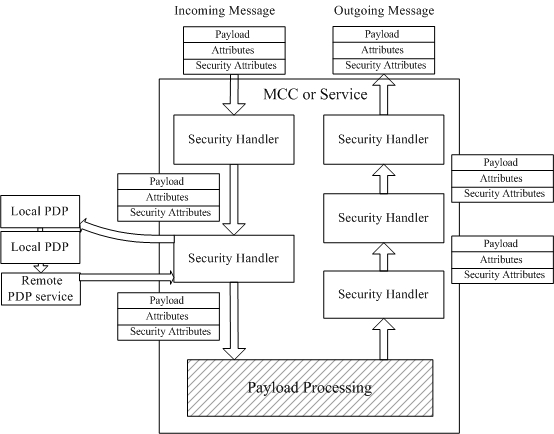
\includegraphics[width=5.7709in,height=4.5209in]{SecurityFrameworkofARC1-img2.jpg}


{\selectlanguage{english}\itshape\color{black}
Figure \stepcounter{Figure}{\theFigure}. There are usually two chains of
SecHandlers inside the MCC or service. Each SecHandler will parse the
Security Attributes which are generated by the upstream MCC/services or
probably upstream SecHandlers in the same or other MCC/Service, and do
message processing or authenticate or authorize the incoming/outgoing
message based on the collected information. The SecHandler can also
change the payload and attributes of Messsage itself. For example, the
Username-Token SecHandler will insert the WSS Username Token [3] into
header part of SOAP message. The PDPs are called by the SecHandlers and
are supposed to make authorization decision. Here the two local PDP and
one remote PDP service is just for demonstration, and one or any number
of PDPs can be configured under each SecHandler.}


\bigskip

[Warning: Draw object ignored]

{\centering\selectlanguage{english}\itshape\color{black}
Figure \stepcounter{Figure}{\theFigure}. Example Echo service is
configured to use two SecHandlers, both responsible for authorization.
First SecHandler uses the identity of client extracted from the
incoming message to map it into local identity like local Linux
username. In this case all clients are mapped to local account
{\textquotedblleft}test{\textquotedblright}. The second one uses two
PDPs: one will compose ARC specific authorization request based on the
Security Attributes collected from
{\textquotedblleft}incoming{\textquotedblright} message and evaluate it
against the ARC specific authorization policy which is defined in local
file {\textquotedblleft}policy.xml{\textquotedblright}; the other will
compare the X509 identity of client extracted from the incoming message
against list of identities stored locally.
\par}

\subsubsection{Interface of SecHandler}
{\selectlanguage{english}\upshape\color{black}
When one component (MCC or service) is loaded according to the
configuration information, the SecHandler under the component and the
plug-ins like PDP which are attached to the SecHandler will be loaded
as well. }

{\selectlanguage{english}\upshape\color{black}
There is one simple interface (see Figure 3) defined in class
SecHandler, which will be called by the containing MCC/Service once
there is message (incoming or outgoing) need to be processed.}

{\centering\selectlanguage{english}\itshape\color{black}
Figure \stepcounter{Figure}{\theFigure}. class SecHandler is an abstract
class which includes a general interface called Handle which uses
Message object as argument. Any security handler implementation should
inherit class SecHandler and implement the interface according to the
actual functionality. The interface only return simple Boolean value,
and any useful information generated during the calling of this
interface should be put into the security attribute of the message, or
put into the payload itself. 
\par}

\begin{center}
\begin{minipage}{3.3752in}
{\selectlanguage{english}\color{black}
\ \ class SecHandler \{}

{\selectlanguage{english}\upshape\color{black}
\ \ \ public:}

{\selectlanguage{english}\upshape\color{black}
\ \ \ \ SecHandler(Arc::Config*) \{\};}

{\selectlanguage{english}\upshape\color{black}
\ \ \ \ virtual \~{}SecHandler() \{\};}

{\selectlanguage{english}\upshape\color{black}
\ \ \ \ virtual bool \textit{Handle}(Arc::Message *msg) = 0;}

{\selectlanguage{english}\color{black}
\ \ \};}
\end{minipage}
\end{center}
{\selectlanguage{english}\upshape\color{black}
Currently, the ARC1 comes with the following four security handler
implemented: }

\liststyleWWviiiNumxiii
\begin{itemize}
\item {\selectlanguage{english}\color{black}
\textit{arc.authz} -- Authorization SecHandler}
\end{itemize}
{\selectlanguage{english}\upshape\color{black}
The \textit{arc.authz} is responsible for calling the interface of
policy decision point and getting back the authorization result, and
then making decision according to this authorization result. There is
one simple interface (see Figure 4) defined in PDP, which will be
called by \textit{arc.authz} if configured inside once there is message
(incoming or outgoing) need to be processed.}

\liststyleWWviiiNumxiii
\begin{itemize}
\item {\selectlanguage{english}\color{black}
\textit{identity.map} -- Identity Mapping SecHandler}
\end{itemize}
{\selectlanguage{english}\upshape\color{black}
The \textit{identity.map} is a specific authorization oriented security
handler. It will map the global identity in the message into local
identity like system username based on the result returned by Policy
Decision Point components.}

\liststyleWWviiiNumxiii
\begin{itemize}
\item {\selectlanguage{english}\color{black}
\textit{delegation.collector} -- Delegation SecHandler}
\end{itemize}
{\selectlanguage{english}\upshape\color{black}
The \textit{delegation.collector} is responsible for collecting the
delegation policy information from the remote proxy credential (proxy
certificate is compatible to RFC3820) inside the message, and putting
this policy into message{\textquoteright}s security attribute for the
usage of other components, such as \ \textit{delegation.pdp}.}

\liststyleWWviiiNumxiii
\begin{itemize}
\item {\selectlanguage{english}\color{black}
\textit{usernametoken.handler} -- UseranemToken SecHandler}
\end{itemize}
{\selectlanguage{english}\upshape\color{black}
The task of the \ \textit{usernametoken.handler} is to generate the
WS-Security Username-Token and add it into header of SOAP message which
is the payload of outgoing message. It can also extract the WS-Security
Username-Token from the header of SOAP message which is the payload of
incoming message.}

\subsubsection[Interface of PDP]{Interface of PDP}
\label{bkm:Ref204009855}{\selectlanguage{english}\upshape\color{black}
Figure 4 shows the definition of abstract class PDP. The implementation
could be some function which implements the interface by composing the
policy evaluation request, evaluating this request against some policy,
and returning the evaluation result, or just by composing the policy
evaluation request, invoking some remote policy decision web service
and getting back the evaluation result.}

{\centering\selectlanguage{english}\itshape\color{black}
Figure \stepcounter{Figure}{\theFigure}. class PDP is an abstract class
which includes a general interface called isPermitted which uses
Message object as argument. Any policy decision point implementation
should inherit class PDP and implement the interface according to the
actual functionality. The interface only return simple Boolean value,
and any useful information generated during the calling of this
interface should be put into the security attribute of the message, or
put into the payload itself.
\par}

\begin{center}
\begin{minipage}{3.8752in}
{\selectlanguage{english}\color{black}
\ \ class PDP \{}

{\selectlanguage{english}\upshape\color{black}
\ \ \ public:}

{\selectlanguage{english}\upshape\color{black}
\ \ \ \ PDP(Arc::Config* cfg) \{ \};}

{\selectlanguage{english}\upshape\color{black}
\ \ \ \ virtual \~{}PDP() \{\};}

{\selectlanguage{english}\upshape\color{black}
\ \ \ \ virtual bool \textit{isPermitted}(Arc::Message *msg) = 0;}

{\selectlanguage{english}\color{black}
\ \ \};}
\end{minipage}
\end{center}
{\selectlanguage{english}\upshape\color{black}
Currently, the ARC1 comes with the following four policy decision point
implementation: }

\liststyleWWviiiNumxiii
\begin{itemize}
\item {\selectlanguage{english}\color{black}
\textit{arc.pdp }{}-- Arc PDP}
\end{itemize}
{\selectlanguage{english}\upshape\color{black}
The Arc PDP will organize the security attributes into the ARC specific
authorization request, call the policy evaluator to evaluate the
request against the policy (which is in ARC specific format)
repository, and get back the evaluation result. See paragraph 3 for
detail information about request schema and policy schema.}

\liststyleWWviiiNumxiii
\begin{itemize}
\item {\selectlanguage{english}\color{black}
\textit{delegtion.pdp} -- Delegation PDP}
\end{itemize}
{\selectlanguage{english}\upshape\color{black}
The Delegation PDP is basically similar to Arc PDP, except it uses the
delegation policy parsed from remote proxy credential by
\textit{delegation.collector}, and evaluates the request against
delegation policy. See section 6for the design idea and use case of
delegation policy in fine-grained identity delegation.}

\liststyleWWviiiNumxiii
\begin{itemize}
\item {\selectlanguage{english}\color{black}
\textit{simplelist.pdp} -- Simplelist PDP}
\end{itemize}
{\selectlanguage{english}\upshape\color{black}
The Simplelist PDP is a simplest implementation of policy decision
point. It will match the identity extracted from the remote credential
(or proxy credential) with local list of permitted identities.}

\liststyleWWviiiNumxiii
\begin{itemize}
\item {\selectlanguage{english}\color{black}
\textit{pdpservice.invoker} -- PDP Service Invoker}
\end{itemize}
{\selectlanguage{english}\upshape\color{black}
The PDP Service Invoker is a client which can be used to invoke the PDP
Service which implements the same functionality as Arc PDP, except that
the evaluation request and response are carried by SOAP message. The
benefit of implementing PDP Service and PDP Service Invoker is that the
policy evaluation engine can be accessed remotely and maintained
centrally.}

\subsection[Policy Evaluation Engine]{Policy Evaluation Engine}
\subsubsection{Design of policy evaluation engine}
{\selectlanguage{english}\upshape\color{black}
The ARC1 defines specific evaluation request and policy schema. Based on
the schema definition, one policy evaluation engine is implemented. The
design principal of policy evaluation engine is generality by which the
implementation of the policy evaluation engine can be easily extended
to adopt some other policy schema, such as XACML policy schema.}

{\selectlanguage{english}\upshape\color{black}
Figure 5 shows the UML class diagram about the policy evaluation engine.
It shows all classes and relations simultaneously for getting the
overall picture. }

{\selectlanguage{english}\upshape\color{black}
The \textit{Evaluator} class is the key class for policy evaluation. It
accepts request evaluates it against loaded policy and returns
evaluation response. }

{\selectlanguage{english}\upshape\color{black}
Three abstract factories - \textit{FnFactory}, \textit{AlgFactory},
\textit{AttributeFactory} - are responsible for creating the
\textit{Function}, \textit{CombiningAlg} and \textit{AttributeValue}
objects correspondingly. The classes inherited from
\textit{CombiningAlg} class take care of implementing various combining
algorithms which define relations between
{\textless}Rule/{\textgreater} elements in policy. The
\textit{AttributeValue} type of classes are used for processing
different types of {\textless}Attribute/{\textgreater} and similar
elements. The \textit{Function} classes take care of comparing
{\textless}Attribute/{\textgreater} elements of request and policy. }

{\selectlanguage{english}\upshape\color{black}
The \textit{Policy} class parses {\textless}Policy/{\textgreater} or
{\textless}Rule/{\textgreater} elements and creates
\ \textit{CombingAlg} objects according to the
{\textless}RuleCombiningAlg/{\textgreater} attribute of
{\textless}Policy/{\textgreater}, \textit{Function} objects according
to the {\textless}Function/{\textgreater} attribute of
{\textless}Attribute/{\textgreater} and \textit{AttributeValue} objects
according to the {\textless}Type/{\textgreater} attribute of
{\textless}Attribute/{\textgreater}. Those objects will be used when
evaluating the request.}

{\selectlanguage{english}\upshape\color{black}
The \textit{Request} class is responsible for parsing
{\textless}Request/{\textgreater} element and creates corresponding
\textit{AttributeValue} objects according to the
{\textless}Type/{\textgreater} attribute of
{\textless}Attribute/{\textgreater}. When evaluating, each
\textit{AttributeValue} in request will be evaluated against
corresponding \textit{AttributeValue} in the policy by using relevant
\textit{Function}.}

{\selectlanguage{english}\upshape\color{black}
Due to extensible architecture of code it is relatively easy to add
support for new types of \ \textit{AttributeValue}, \textit{Function
and CombingAlg} objects in this way supporting various types of XML
based policy languages.}


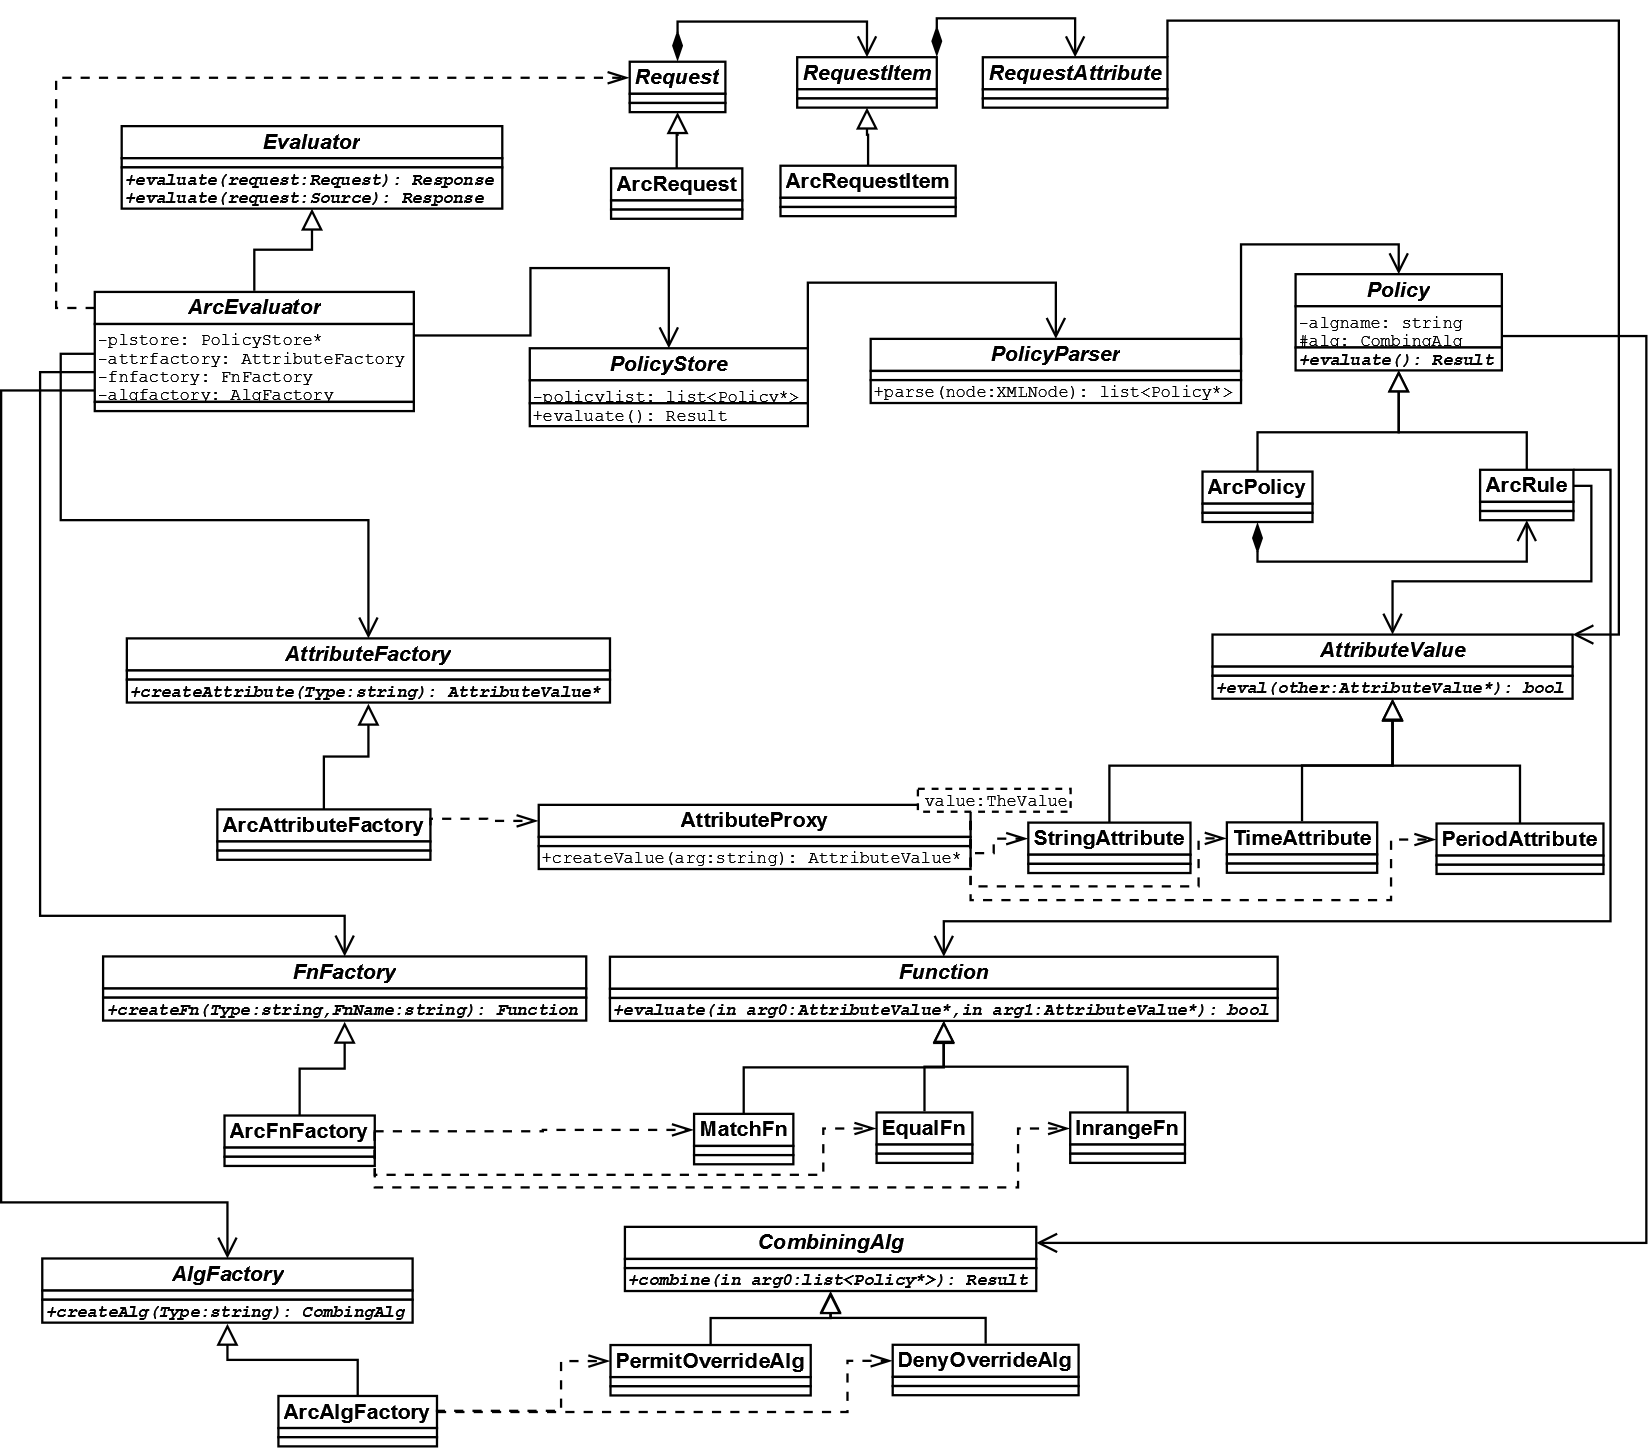
\includegraphics[width=0.0161in,height=0.0161in]{SecurityFrameworkofARC1-img3.png}

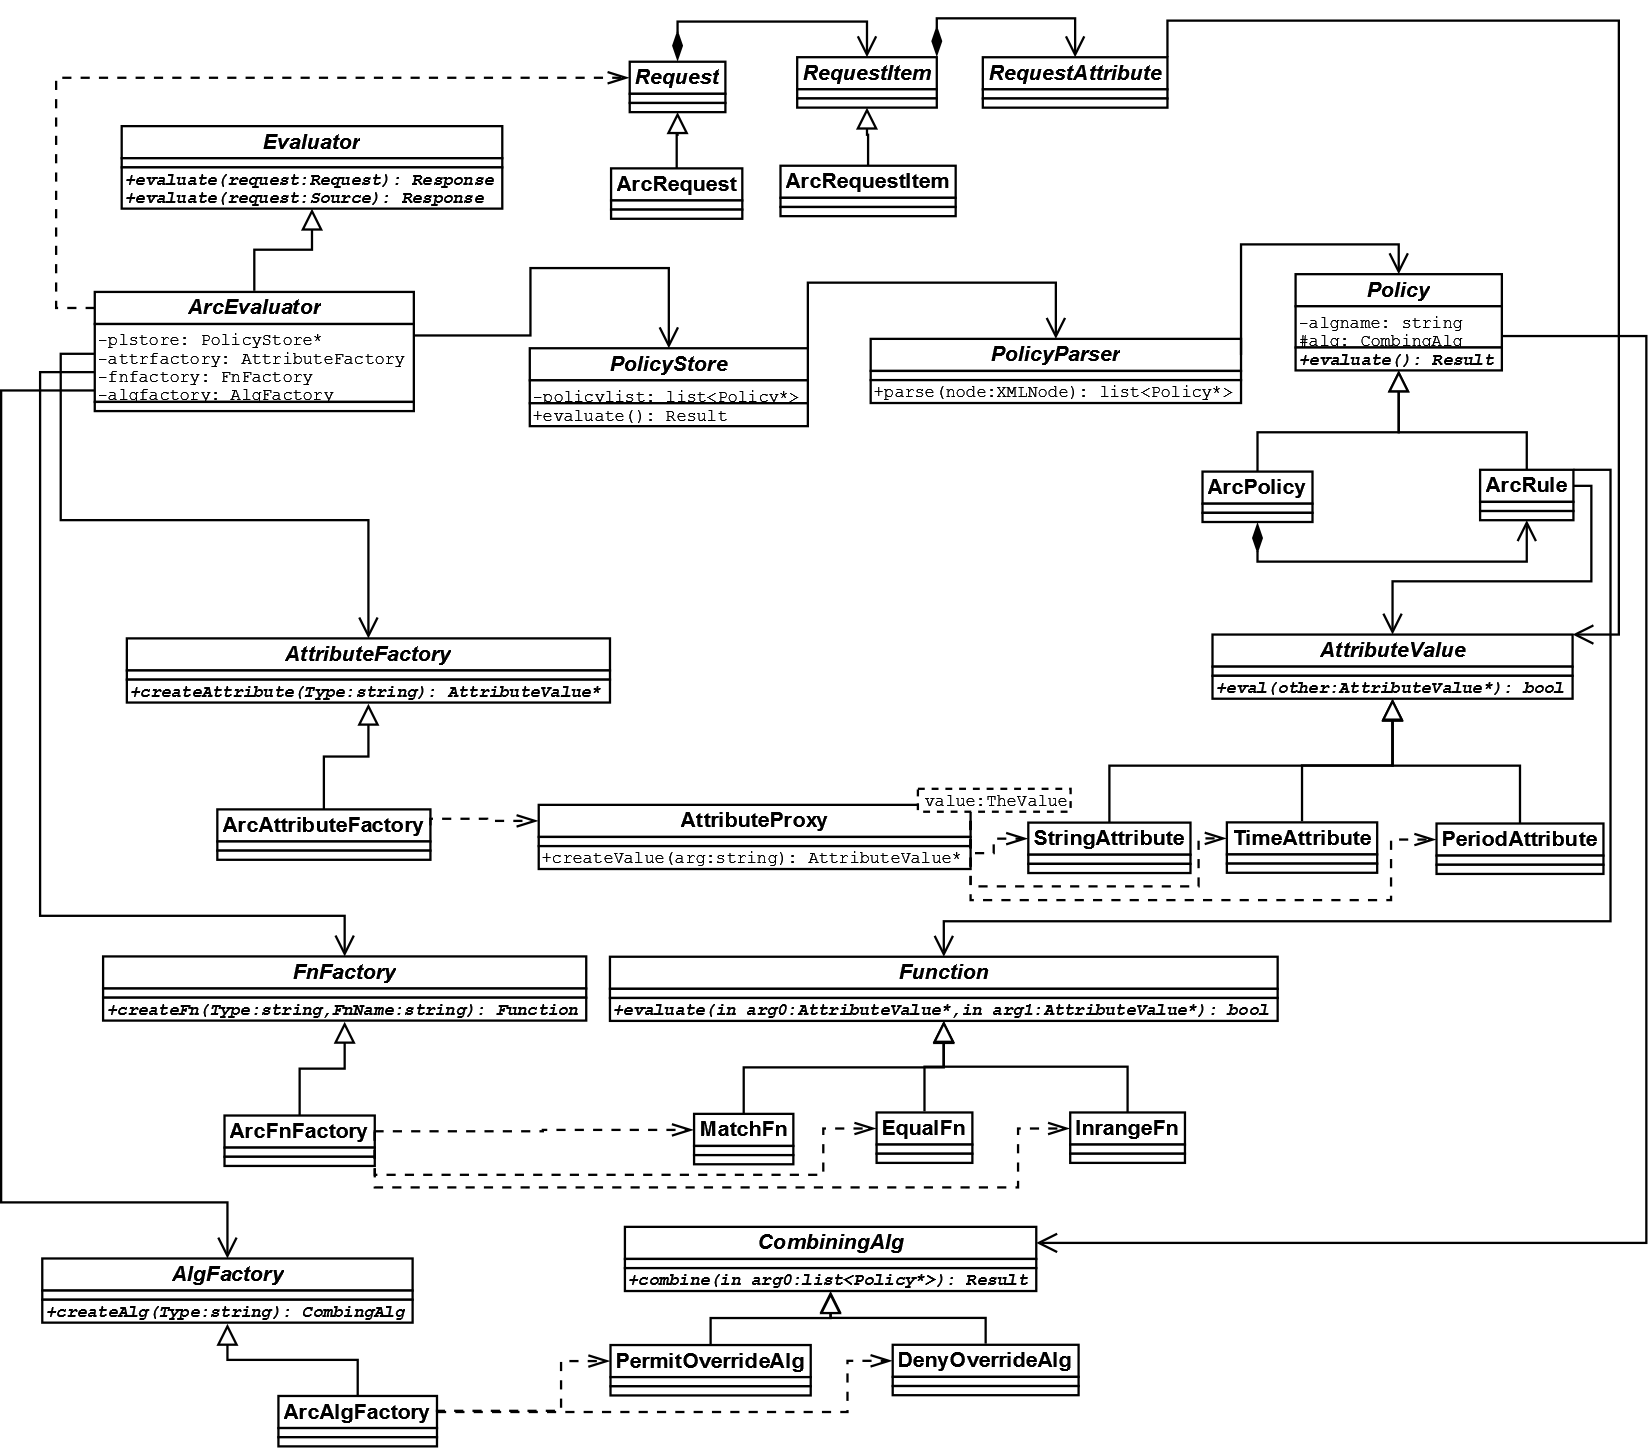
\includegraphics[width=0.0161in,height=0.0161in]{SecurityFrameworkofARC1-img4.png}

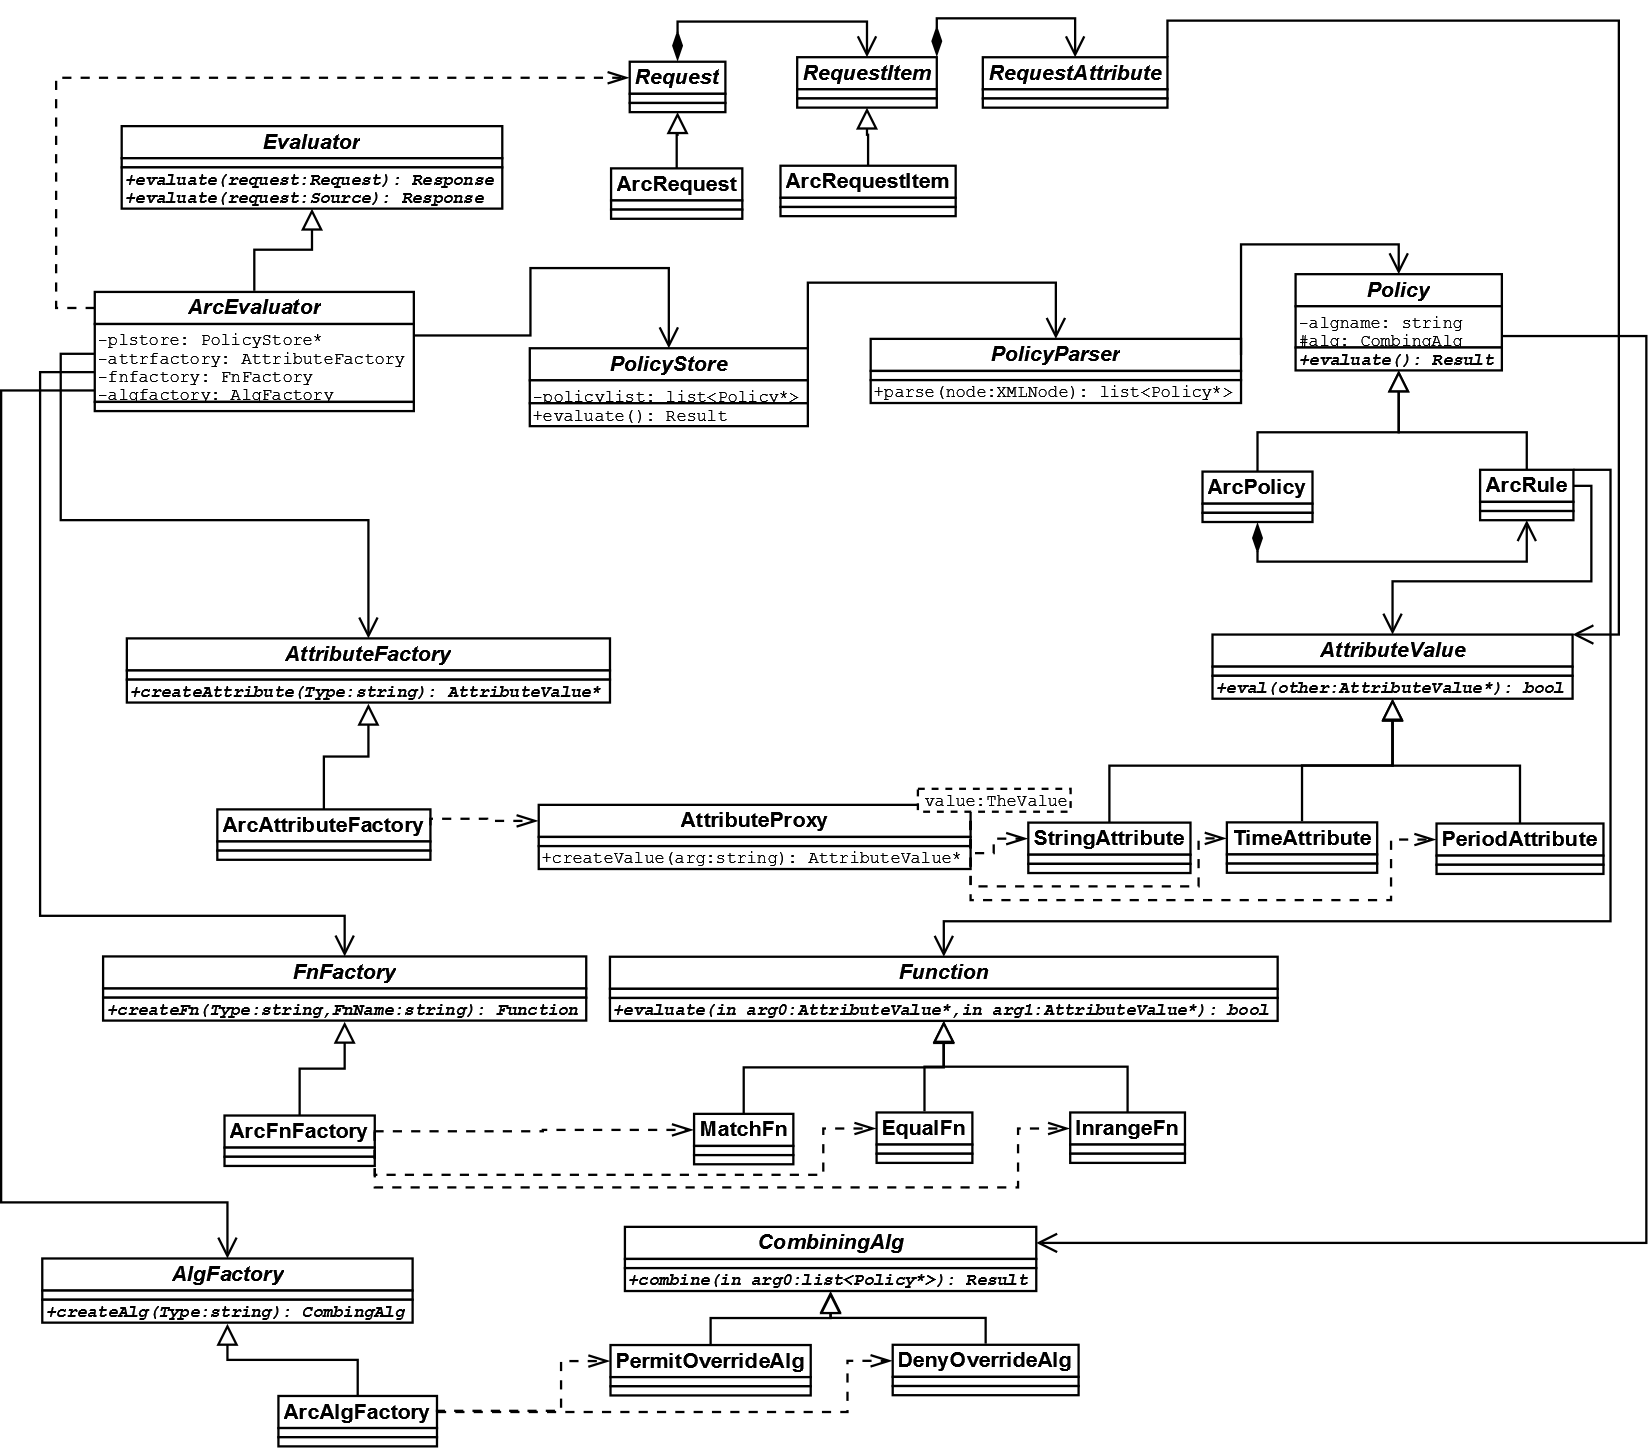
\includegraphics[width=0.0161in,height=0.0161in]{SecurityFrameworkofARC1-img5.png}

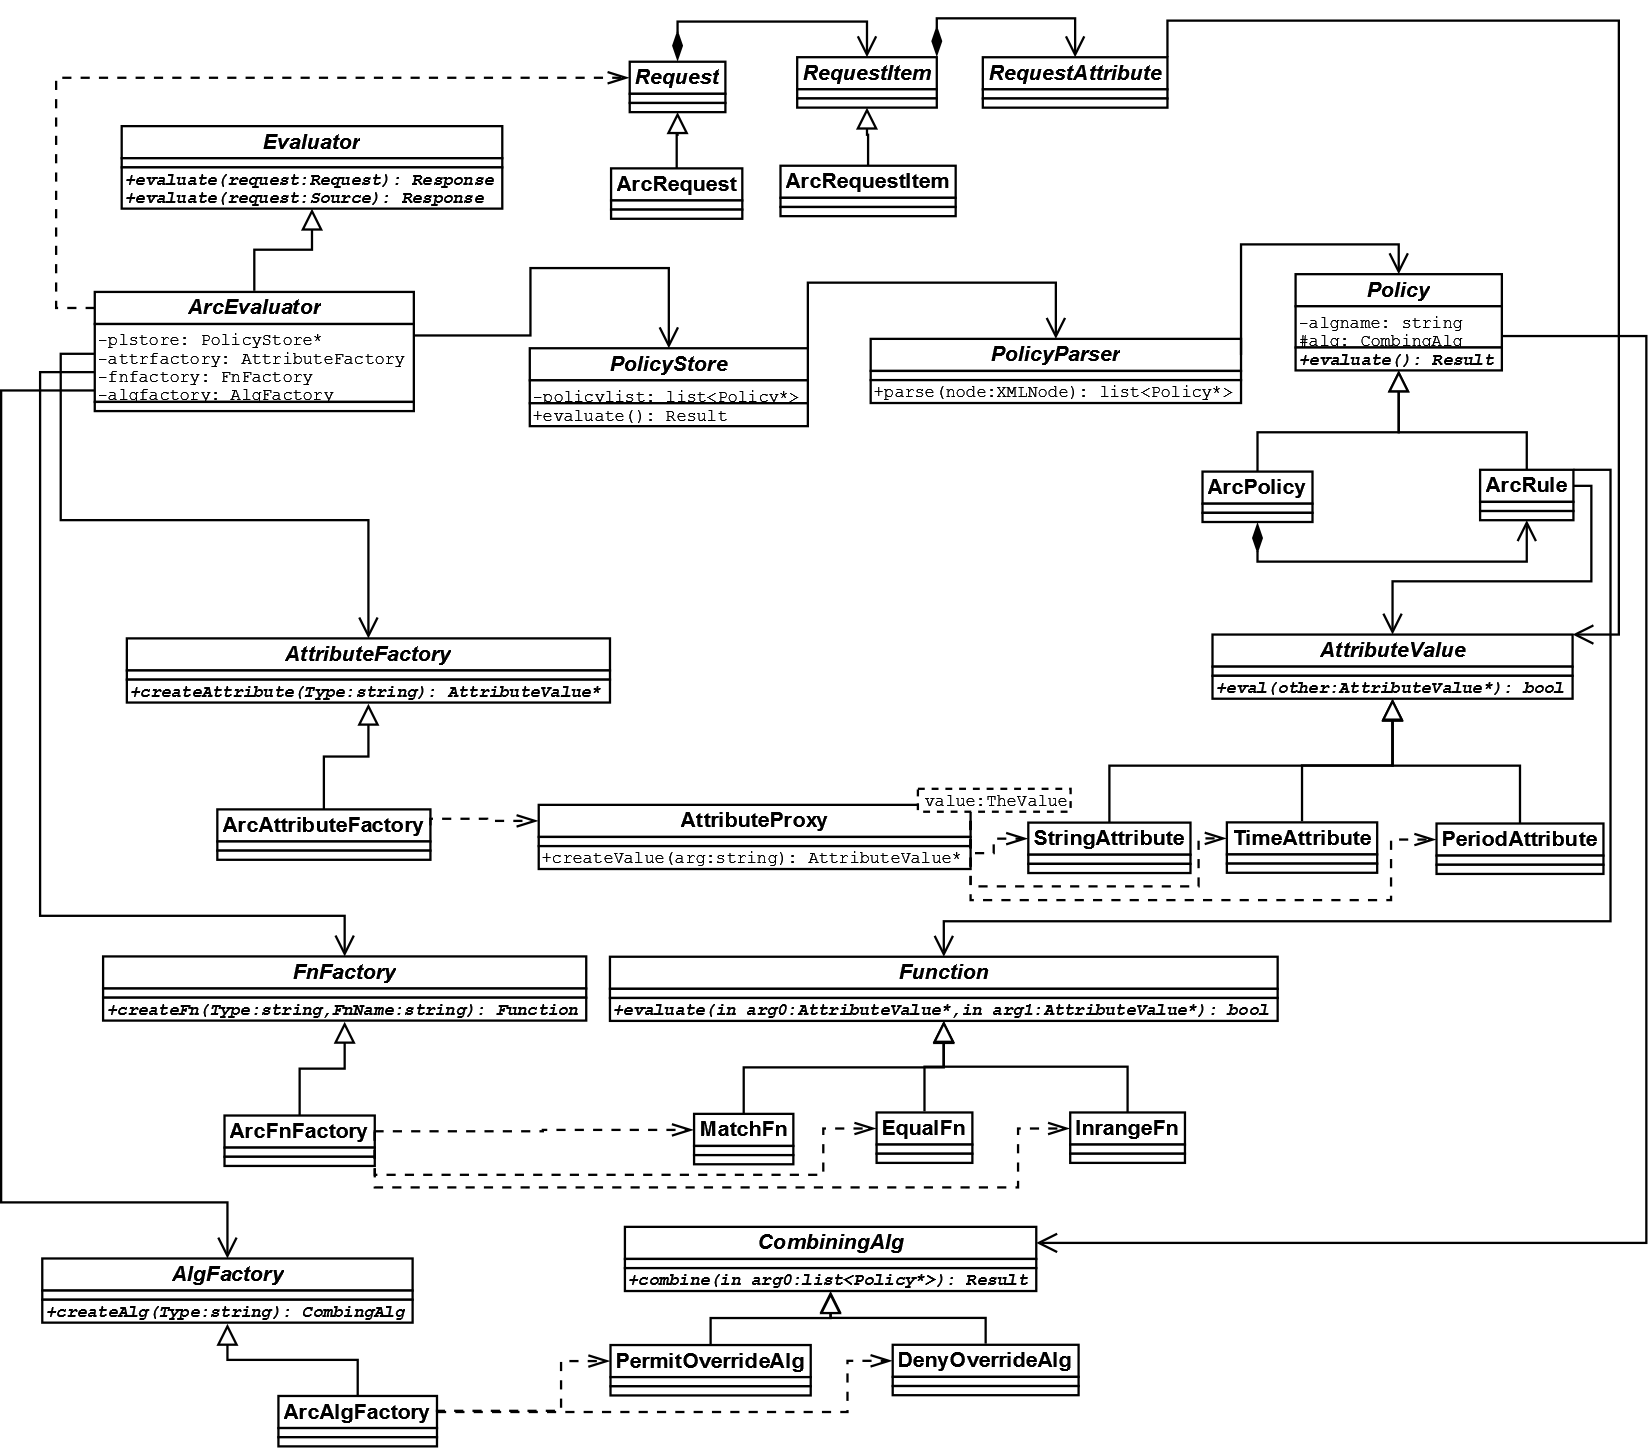
\includegraphics[width=5.9709in,height=6.3957in]{SecurityFrameworkofARC1-img6.png}


{\centering\selectlanguage{english}\itshape\color{black}
Figure \stepcounter{Figure}{\theFigure}. The UML class diagram of the
classes inside policy evaluation engine. 
\par}

\subsubsection{Schemas for policy evaluation engine}
{\selectlanguage{english}\upshape\color{black}
The schema for ARC Policy is available at}

{\selectlanguage{english}\upshape\color{black}
\url{http://svn.nordugrid.org/trac/nordugrid/browser/arc1/trunk/src/hed/pdc/arcpdp/Policy.xsd}
.}

{\selectlanguage{english}\color{black}
The hierarchy tree of ARC Policy is show below (numbers show
multiplicity of elements)}

{\selectlanguage{english}\itshape\color{black}
Policy (1)}

{\selectlanguage{english}\itshape\color{black}
 Rule (1-)}

{\selectlanguage{english}\itshape\color{black}
  Subjects (1)}

{\selectlanguage{english}\itshape\color{black}
   Subject (1-)}

{\selectlanguage{english}\itshape\color{black}
    Attribute (1-)}

{\selectlanguage{english}\itshape\color{black}
   Resources (0-1)}

{\selectlanguage{english}\itshape\color{black}
   Resource (1-)}

{\selectlanguage{english}\itshape\color{black}
  Actions (0-1)}

{\selectlanguage{english}\itshape\color{black}
   Action (1-)}

{\selectlanguage{english}\itshape\color{black}
  Conditions (0-1)}

{\selectlanguage{english}\itshape\color{black}
   Condition (1-)}

{\selectlanguage{english}\itshape\color{black}
    Attribute (1-)}

{\selectlanguage{english}\upshape\color{black}
The schema for ARC Request is available at \ }

{\selectlanguage{english}\upshape\color{black}
\url{http://svn.nordugrid.org/trac/nordugrid/browser/arc1/trunk/src/hed/pdc/arcpdp/Request.xsd}
.}

{\selectlanguage{english}\upshape\color{black}
The hierarchy tree of ARC Request is show below (numbers show
multiplicity of elements)}

{\selectlanguage{english}\itshape\color{black}
Request (1)}

{\selectlanguage{english}\itshape\color{black}
 RequestItem (1-)}

{\selectlanguage{english}\itshape\color{black}
  Subject (1-)}

{\selectlanguage{english}\itshape\color{black}
   SubjectAttribute (1-)}

{\selectlanguage{english}\itshape\color{black}
  Resource (0-)}

{\selectlanguage{english}\itshape\color{black}
  Action (0-)}

{\selectlanguage{english}\itshape\color{black}
  Context (0-)}

{\selectlanguage{english}\itshape\color{black}
   ContextAttribute (1-)}

{\selectlanguage{english}\upshape\color{black}
The schema for ARC Response is available at}

{\selectlanguage{english}\upshape\color{black}
\url{http://svn.nordugrid.org/trac/nordugrid/browser/arc1/trunk/src/hed/pdc/arcpdp/Response.xsd}
.}

{\selectlanguage{english}\upshape\color{black}
The ARC Response is not used directly in code. It is in use by PDP
Service which provides remote evaluation of policies. }

\subsubsection{Basic Elements of Policy}
{\selectlanguage{english}\upshape\color{black}
There are 2 basic objects - {\textquotedbl}policy{\textquotedbl} and
{\textquotedbl}request{\textquotedbl}. There is 1 main actor -
Evaluator. Curretly there are two types of elements in policy: Policy
and Rule. Policy element is made of Rule elements.}

{\color{black}
Evaluator matches request to policy and produces one of 4 following
results:}

\liststyleWWviiiNumxxi
\begin{itemize}
\item {\selectlanguage{english}\color{black}
\textbf{PERMIT} - policy explicitely permits activity specified in
request because request matches some part of policy and corresponding
effect specified in policy is PERMIT. }
\end{itemize}
{\bfseries\itshape\color{black}
Example: }

{\selectlanguage{english}\upshape\color{black}
\textbf{\textit{\ \ \ \ \ \ }}\textbf{\textit{Rule: }}\textit{PERMIT
person ALICE to PLAY in place called WONDERLAND}}

{\selectlanguage{english}\upshape\color{black}
\textbf{\textit{\ \ \ \ \ \ }}\textbf{\textit{Request: }}\textit{person
ALICE wants to PLAY in place called WONDERLAND}}

\liststyleWWviiiNumxxi
\begin{itemize}
\item {\selectlanguage{english}\color{black}
\textbf{DENY} - policy explicitely denies activity specified in Request
because Request matches some part of policy and corresponding effect
specified in policy is DENY.}
\end{itemize}
{\bfseries\itshape\color{black}
Example:}

{\selectlanguage{english}\upshape\color{black}
\textbf{\textit{\ \ \ \ \ \ }}\textbf{\textit{Rule: DENY }}\textit{fruit
APPLE to GROW on PEACH tree}}

{\selectlanguage{english}\upshape\color{black}
\textbf{\textit{\ \ \ \ \ \ }}\textbf{\textit{Request}}\textit{: fruit
APPLE to be GROWN on PEACH tree}}

\liststyleWWviiiNumxxi
\begin{itemize}
\item {\selectlanguage{english}\color{black}
\textbf{INDETERMINATE} - request has some part which does not correspond
to policy.}
\end{itemize}
{\bfseries\itshape\color{black}
Example: }

{\selectlanguage{english}\upshape\color{black}
\textit{\ \ \ \ \ \ }\textbf{\textit{Rule}}\textit{: DENY fruit APPLE to
GROW on PEACH tree}}

{\selectlanguage{english}\upshape\color{black}
\textit{\ \ \ \ \ \ }\textbf{\textit{Request}}\textit{: fruit APPLE to
be GROWN on WHEAT ground}}

{\selectlanguage{english}\upshape\color{black}
\textit{\ \ \ \ \ \ }\textbf{\textit{Request}}\textit{: flower SUNFLOWER
to be grown on PEACH tree}}

{\selectlanguage{english}\upshape\color{black}
\textbf{\textit{Explaination}}: Here, it is not possible to obtain any
matching result - neither positive (DENY or PERMIT) nor negative
(NOT\_APPLICABLE, see below)}

{\color{black}
In the request, the {\textquotedbl}ground{\textquotedbl} is completely
uncomparable to the {\textquotedbl}tree{\textquotedbl} in policy. One
can compare {\textquotedbl}PEACH tree{\textquotedbl} and
{\textquotedbl}APPLE tree{\textquotedbl} because they are both
{\textquotedbl}tree{\textquotedbl}; But it is impossible to compare
{\textquotedbl}PEACH tree{\textquotedbl} and {\textquotedbl}WHEAT
ground{\textquotedbl} becaue they of different kind (Policy is about
tree and Request is about ground).}

{\color{black}
In a similar way one can{\textquotesingle}t compare {\textquotedbl}fruit
APPLE{\textquotedbl} and {\textquotedbl}flower SUNFLOWER{\textquotedbl}
(here policy is about fruits and Request is about flower).}

{\color{black}
Any other situation which makes it impossibile to compare two attributes
will also cause {\textquotedbl}INDETERMINATE{\textquotedbl}.}


\bigskip

\liststyleWWviiiNumxxi
\begin{itemize}
\item {\selectlanguage{english}\color{black}
\textbf{NOT\_APPLICABLE} - all parts of the Request have corresponding
parts in the Policy, but some value of those parts are not the same.
Hence request does not match policy.}
\end{itemize}
{\bfseries\itshape\color{black}
Example:}

{\selectlanguage{english}\upshape\color{black}
\textit{\ \ \ \ \ \ }\textbf{\textit{Rule}}\textit{: DENY fruit APPLE to
GROW on PEACH tree}}

{\selectlanguage{english}\upshape\color{black}
\textit{\ \ \ \ \ \ }\textbf{\textit{Request}}\textit{: fruit APPLE to
be GROWN on APPLE tree }}

{\selectlanguage{english}\upshape\color{black}
\textit{\ \ \ \ \ \ }\textbf{\textit{Request}}\textit{: fruit ORANGE to
be GROWN on PEACH tree }}

{\selectlanguage{english}\upshape\color{black}
\textit{\ \ \ \ \ \ }\textbf{\textit{Request}}\textit{: fruit ORANGE to
be GROWN on APPLE tree }}

{\color{black}
Explanation: for each part of the Request evaluator can find relevant
part in the Policy - both Policy and Request are about fruit and tree.
But the values do not match.}

{\color{black}
If it is required to reduce evaluation results to boolean value PERMIT
maps to TRUE and rest of results to FALSE.}

{\selectlanguage{english}\upshape\color{black}
\textbf{\textit{Note}}\textit{: It would be useful to make it possible
to specify secondary effect which would become }active in case Request
is NOT\_APPLICABLE. For example:}

{\itshape\color{black}
DENY fruit APPLE to GROW on PEACH tree otherwise PERMIT}

{\color{black}
But one should be careful because example above would allow fruit PLUMS
to grow on APPLE trees :)}

{\color{black}
This kind of requirement can be supported by using the algorithm between
policies. \ For example, in case of above scenario, we can use some
algorithm like {\textquotedbl}Permit-if-notapplicable{\textquotedbl}.
See below the {\textquotedbl}Policy matching{\textquotedbl} part for
more explaination. \ }

\subsubsection{Policy MAtching}
{\selectlanguage{english}\upshape\color{black}
Policy is made of Rule elements. Request is evaluated against each Rule.
Each evaluation produces same results as policy evaluation described
above. The results from all Rules are then combined in order to produce
final result for whole policy. Results Combining Algorithm is specified
in Policy. There are 26 algorithms currently:}

\liststyleWWviiiNumxxi
\begin{itemize}
\item {\selectlanguage{english}\color{black}
\textbf{\textit{Deny-Overrides}} - this is default if no algorithm
specified.}

\begin{itemize}
\item {\color{black}
If there is at least one DENY in results final result is DENY.}
\item {\color{black}
Otherwise if there is at least one PERMIT, the final result is PERMIT.}
\item {\color{black}
Otherwise if there is at least one NOT\_APPLICABLE final result is
NOT\_APPLICABLE.}
\item {\color{black}
Otherwise final result is INDETERMINATE.}
\end{itemize}
\end{itemize}
{\selectlanguage{english}\upshape\color{black}
\textbf{NOTE}\textbf{: CHECK if algorithm description is correct}}

{\color{black}
Special case is Policy wih no rules. Probably such policy shoudl be
treated as always producing DENY.}

{\bfseries\color{black}
Discussion}

{\itshape\color{black}
If there is no Rule under Policy, it means no restriction from this
Policy, what exactly shoud the Policy give? DENY or NOT\_APPLICABLE?}

{\itshape\color{black}
It seems to be more logical to produce INDETERMINATE because there is no
rule with elements which could be compared to request.}

\liststyleWWviiiNumxxi
\begin{itemize}
\item {\bfseries\itshape\color{black}
Permit-Overrides.}

\begin{itemize}
\item {\color{black}
If there is at least one PERMIT in results final result is PERMIT.}
\item {\color{black}
Otherwise if there is at least one DENY the final result is DENY.}
\item {\color{black}
Otherwise if there is at least one NOT\_APPLICABLE final result is
NOT\_APPLICABLE.}
\item {\color{black}
Otherwise final result is INDETERMINATE.}
\end{itemize}
\end{itemize}
{\color{black}
Special case is Policy wih no rules. Probably such policy should be
treated as always producing DENY.}

{\bfseries\color{black}
NOTE: CHECK if algorithm description is correct}

{\bfseries\color{black}
Discussion}

{\itshape\color{black}
Question? The same as above.}

\liststyleWWviiiNumxxi
\begin{itemize}
\item {\bfseries\itshape\color{black}
Ordered algorithms.}
\end{itemize}
{\selectlanguage{english}\color{black}
These specify priorities for all four possible results. Their names look
like Result1-Result2-Result3-Result4 with Result\# naming result types,
for example Permit-Deny-NotApplicable-Indeterminate. The results are
combined in following way:}

\liststyleWWviiiNumxxi
\begin{itemize}
\item \begin{itemize}
\item {\color{black}
If there is at least one result of Result1 type then final result is
Result1.}
\item {\color{black}
Otherwise if there is at least one result of Result2 type then final
result is Result2.}
\item {\color{black}
Otherwise if there is at least one result of Result3 type then final
result is Result3.}
\item {\color{black}
Otherwise final result is Result4.}
\end{itemize}
\end{itemize}
{\color{black}
There are 24 possible combinations of those algorithms.}

{\selectlanguage{english}\upshape\color{black}
\textbf{Note:} It would be useful to have more combining algorithms. For
example }

\liststyleWWviiiNumxxi
\begin{itemize}
\item {\selectlanguage{english}\color{black}
Permit-if-notapplicable - the use case could be {\textquotedbl}DENY
fruit APPLE to GROW on PEACH tree otherwise PERMIT{\textquotedbl}. In
this case there is only one Rule under Policy, and this Rule is with
{\textquotedbl}Deny{\textquotedbl} effect. }

\begin{itemize}
\item {\color{black}
If this Rule gives DENY in results, final result is DENY.}
\item {\color{black}
Otherwise if this Rule gives NOT\_APPLICABLE, final result is PERMIT.}
\item {\color{black}
Otherwise final result is INDETERMINATE. }
\end{itemize}
\item {\selectlanguage{english}\color{black}
{\textquotedblleft}Permit-if-allPermit{\textquotedbl} - Permit if all
the Rules gives Permit, this algorithm is useful in case if we are
collecting different policies from a few sources, and we want the
request to satisfy all of them.}

\begin{itemize}
\item {\color{black}
If all of the Rule give PERMIT, the final result is PERMIT.}
\item {\color{black}
Otherwise if there is at least one DENY the final result is DENY.}
\item {\color{black}
Otherwise if there is at least one NOT\_APPLICABLE final result is
NOT\_APPLICABLE.}
\item {\color{black}
Otherwise final result is INDETERMINATE.}
\end{itemize}
\item {\color{black}
OnlyOneApplicable}

\begin{itemize}
\item {\color{black}
If there is one gives INDETERMINATE, final result INDETERMINATE is given
immediately.}
\item {\color{black}
Otherwise if there is exactly only one gives applicable result (DENY or
PERMIT), final result is as this result.}
\item {\color{black}
Otherwise if there is more than one gives applicable result, final
result is INDTERMINATE.}
\item {\selectlanguage{english}\color{black}
Otherwise final result is NOT\_APPLICABLE.}
\end{itemize}
\end{itemize}
{\color{black}
This algorithm makes sure that only one Rule is selected when making
decision.}

\liststyleWWviiiNumxvii
\begin{itemize}
\item {\color{black}
FirstApplicable}

\begin{itemize}
\item {\color{black}
If there is one give DENY, PERMIT or INDETERMINATE result, final result
is given immediately as this result.}
\item {\color{black}
Otherwise final result is NOT\_APPLICABLE.}
\end{itemize}
\end{itemize}
\subsubsection{Request Structure}
{\selectlanguage{english}\upshape\color{black}
Request is made of RequestItem elements. Each RequestItem is evaluated
against Policy Rule and for each evaluation separate result is
generated as described above.RequestItem is made of 4 elements:}

{\color{black}
Subject - represents entity requesting specified action}

\liststyleWWviiiNumxix
\begin{itemize}
\item {\color{black}
Resource - destination/object of the action}
\item {\color{black}
Action - specifies what has to be done on resource}
\item {\color{black}
Context - for additional information which does not fit anywhere else,
like the current time.}
\end{itemize}
{\color{black}
Effectively RequestItem may have only one Subject, one Resource, one
Action and one Context. If there are more than one element of any kind
of sub-elelemt, then in the evaluator this RequestItem is split into
several items containing all possible permutations and results are
obtained for every item separately. How results are combined will be
explained later.}

{\color{black}
Additionally Subject could contain sub-elements SubjectAttribute. Those
are meant to represent different kinds of requesters{\textquotesingle}
identities. Example:}

\liststyleWWviiiNumxviii
\begin{itemize}
\item {\color{black}
Subject}

\begin{itemize}
\item {\color{black}
SubjectAttribute: name is ALICE}
\item {\color{black}
SubjectAttribute: age is YOUNG}
\item {\color{black}
SubjectAttribute: gender is GIRL}
\end{itemize}
\end{itemize}
{\color{black}
Context could also be made of ContextAttribute elements in the same way
as Subject.}

{\color{black}
The following is an example of the Request:}

{\itshape\color{black}
{\textless}Request
xmlns={\textquotedbl}http://www.nordugrid.org/schemas/request-arc{\textquotedbl}{\textgreater}}

{\selectlanguage{english}\color{black}
\textit{\ }\textit{{\textless}RequestItem{\textgreater}}}

{\selectlanguage{english}\color{black}
\textit{\ \ \ }\textit{{\textless}Subject{\textgreater}}}

{\selectlanguage{english}\color{black}
\textit{\ \ \ \ \ \ }\textit{{\textless}SubjectAttribute
AttributeId={\textquotedbl}urn:knowarc:x509:identity{\textquotedbl}{\textgreater}/O=KnowARC/OU=UiO/CN=Physicist{\textless}/SubjectAttribute{\textgreater}}}

{\selectlanguage{english}\color{black}
\textit{\ \ \ \ \ \ }\textit{{\textless}SubjectAttribute
AttributeId={\textquotedbl}urn:knowarc:voms:attribute{\textgreater}knowarc:atlasuser{\textless}/SubjectAttribute{\textgreater}}}

{\selectlanguage{english}\color{black}
\textit{\ \ \ }\textit{{\textless}/Subject{\textgreater}}}

{\selectlanguage{english}\color{black}
\textit{\ \ \ }\textit{{\textless}Subject
AttributeId={\textquotedbl}urn:knowarc:shibboleth:attribute{\textquotedbl}{\textgreater}member{\textless}/Subject{\textgreater}}}

{\selectlanguage{english}\color{black}
\textit{\ \ \ }\textit{{\textless}Action
AttributeId={\textquotedbl}urn:knowarc:fileoperation{\textquotedbl}{\textgreater}Read{\textless}/Action{\textgreater}}}

{\selectlanguage{english}\color{black}
\textit{\ \ \ }\textit{{\textless}Resource
AttributeId={\textquotedbl}urn:knowarc:fileidentity{\textgreater}file:///home/test{\textless}/Resource{\textgreater}}}

{\selectlanguage{english}\color{black}
\textit{\ \ \ }\textit{{\textless}Context
AttributeId={\textquotedbl}urn:knowarc:time{\textquotedbl}
Type={\textquotedbl}time{\textquotedbl}{\textgreater}2008-09-15T20:30:20{\textless}/Context{\textgreater}}}

{\selectlanguage{english}\color{black}
\textit{\ }\textit{{\textless}/RequestItem{\textgreater}}}

{\itshape\color{black}
{\textless}/Request{\textgreater}}

{\selectlanguage{english}\upshape\color{black}
While evaluating this RequestItem will be split into two RequestItems:}

{\itshape\color{black}
{\textless}Request
xmlns={\textquotedbl}http://www.nordugrid.org/schemas/request-arc{\textquotedbl}{\textgreater}}

{\selectlanguage{english}\color{black}
\textit{\ }\textit{{\textless}RequestItem{\textgreater}}}

{\selectlanguage{english}\color{black}
\textit{\ \ \ }\textit{{\textless}Subject{\textgreater}}}

{\selectlanguage{english}\color{black}
\textit{\ \ \ \ \ \ }\textit{{\textless}SubjectAttribute
AttributeId={\textquotedbl}urn:knowarc:x509:identity{\textquotedbl}{\textgreater}/O=KnowARC/OU=UiO/CN=Physicist{\textless}/SubjectAttribute{\textgreater}}}

{\selectlanguage{english}\color{black}
\textit{\ \ \ \ \ \ }\textit{{\textless}SubjectAttribute
AttributeId={\textquotedbl}urn:knowarc:voms:attribute{\textgreater}knowarc:atlasuser{\textless}/SubjectAttribute{\textgreater}}}

{\selectlanguage{english}\color{black}
\textit{\ \ \ }\textit{{\textless}/Subject{\textgreater}}}

{\selectlanguage{english}\color{black}
\textit{\ \ \ }\textit{{\textless}Action
AttributeId={\textquotedbl}urn:knowarc:fileoperation{\textquotedbl}{\textgreater}Read{\textless}/Action{\textgreater}}}

{\selectlanguage{english}\color{black}
\textit{\ \ \ }\textit{{\textless}Resource
AttributeId={\textquotedbl}urn:knowarc:fileidentity{\textgreater}file:///home/test{\textless}/Resource{\textgreater}}}

{\selectlanguage{english}\color{black}
\textit{\ \ \ }\textit{{\textless}Context
AttributeId={\textquotedbl}urn:knowarc:time{\textquotedbl}
Type={\textquotedbl}time{\textquotedbl}{\textgreater}2008-09-15T20:30:20{\textless}/Context{\textgreater}}}

{\selectlanguage{english}\color{black}
\textit{\ }\textit{{\textless}/RequestItem{\textgreater}}}

{\selectlanguage{english}\color{black}
\textit{\ }\textit{{\textless}RequestItem{\textgreater}}}

{\selectlanguage{english}\color{black}
\textit{\ \ \ }\textit{{\textless}Subject
AttributeId={\textquotedbl}urn:knowarc:shibboleth:attribute{\textquotedbl}{\textgreater}member{\textless}/Subject{\textgreater}}}

{\selectlanguage{english}\color{black}
\textit{\ \ \ }\textit{{\textless}Action
AttributeId={\textquotedbl}urn:knowarc:fileoperation{\textquotedbl}{\textgreater}Read{\textless}/Action{\textgreater}}}

{\selectlanguage{english}\color{black}
\textit{\ \ \ }\textit{{\textless}Resource
AttributeId={\textquotedbl}urn:knowarc:fileidentity{\textgreater}file:///home/test{\textless}/Resource{\textgreater}}}

{\selectlanguage{english}\color{black}
\textit{\ \ \ }\textit{{\textless}Context
AttributeId={\textquotedbl}urn:knowarc:time{\textquotedbl}
Type={\textquotedbl}time{\textquotedbl}{\textgreater}2008-09-15T20:30:20{\textless}/Context{\textgreater}}}

{\selectlanguage{english}\color{black}
\textit{\ }\textit{{\textless}/RequestItem{\textgreater}}}

{\itshape\color{black}
{\textless}/Request{\textgreater}}

{\selectlanguage{english}\upshape\color{black}
The following means this Subject possesses both of these Attributes.}

{\selectlanguage{english}\color{black}
\textit{\ \ \ }\textit{{\textless}Subject{\textgreater}}}

{\selectlanguage{english}\color{black}
\textit{\ \ \ \ \ \ }\textit{{\textless}SubjectAttribute
AttributeId={\textquotedbl}urn:knowarc:x509:identity{\textquotedbl}{\textgreater}/O=KnowARC/OU=UiO/CN=Physicist{\textless}/SubjectAttribute{\textgreater}}}

{\selectlanguage{english}\color{black}
\textit{\ \ \ \ \ \ }\textit{{\textless}SubjectAttribute
AttributeId={\textquotedbl}urn:knowarc:voms:attribute{\textgreater}knowarc:atlasuser{\textless}/SubjectAttribute{\textgreater}}}

{\selectlanguage{english}\color{black}
\textit{\ \ \ }\textit{{\textless}/Subject{\textgreater}}}

{\color{black}
However, the following means two Subject each of which possesses one
Attribute.}

{\selectlanguage{english}\color{black}
\textit{\ \ \ }\textit{{\textless}Subject
AttributeId={\textquotedbl}urn:knowarc:x509:identity{\textquotedbl}{\textgreater}/O=KnowARC/OU=UiO/CN=Physicist{\textless}/Subject{\textgreater}}}

{\selectlanguage{english}\color{black}
\textit{\ \ \ }\textit{{\textless}Subject
AttributeId={\textquotedbl}urn:knowarc:voms:attribute{\textgreater}knowarc:atlasuser{\textless}/Subject{\textgreater}}}

{\color{black}
The {\textquotedbl}Type{\textquotedbl} xml-attribute is for
distinguishing how to process the xml-node value, which is critical
when evaluate two value from request side and policy side because
different type requires different evaluating/comparing approach. The
default {\textquotedbl}Type{\textquotedbl} is
{\textquotedbl}string{\textquotedbl}, in this case (also with the
{\textquotedbl}Function{\textquotedbl} xml-attribute on the policy side
is {\textquotedbl}equal{\textquotedbl}, which will be explained later),
each letters of these two values will be compared one by one when
evaluating them.}

{\color{black}
The {\textquotedbl}AttributeId{\textquotedbl} xml-attribute is for
evaluator to find the Attribute with AttributeId from the request side
which corresponds to the Attribute with the same AttributeId on the
policy side. Only if two Attributes{\textquotesingle} AttributeId are
equal, the evaluator will then compare the value.}

{\color{black}
Each RequestItem will be sequencialy and independently evaluated against
policy/policies. So for one Request (including few RequestItems), some
RequestItem could get positive evaluation result (PERMIT) from policy
engine, others could get negative evaluation result (DENY,
NOT\_APPLICABLE, INDETERMINATE).}

{\color{black}
It is up to policy decision point to make final decision according to
the evaluation results returned by evaluator, and the evaluator itself
can not give this kind of final decision.}

{\selectlanguage{english}\upshape\color{black}
\textbf{NOTE: This probably should be changed because evaluator is fed
with complete policy and complete request. Hence it is illogical that
it retu}\textbf{rns multiple decisions.}}

{\color{black}
Basically the policy decision point will feed policy engine with
request, get back evaluation results, }

{\color{black}
and make final decision.}


\bigskip

\subsubsection{Rule Composition and Matching}
{\selectlanguage{english}\upshape\color{black}
Policy rule is made of 4 elements - Subjects, Resources, Actions,
Conditions (See the following example). Those are only used to group
multiple elements Subject, Resource, Action, Condition. For instance,
you can merge two Rules with the same Resources, Actions, Conditions,
and the same {\textquotedbl}Effect{\textquotedbl} but different
Subjects into one Rule.}

{\selectlanguage{english}\upshape\color{black}
\textbf{NOTE: That is strange. Why do we need }\textbf{Rule at all?}}

{\selectlanguage{english}\upshape\color{black}
There is no logical relationship between Subject, which means you can
split one Rule into two Subject (under Subjects) into two Rule (each of
which has one Subject (under Subjects)).From now only later ones
(Subjects with only one Subject as sub-element, and the same for
others) are described. Their meaning is same as in request with
Condition corresponding to Context. Subject and Condition elements are
also made of Attributes. All elements may be present more than one
time. During procedure of matching each element in RequestItem is
matched against all elements of same kind in Policy - Subject is
matched to Subject, Resource to Resource, etc. For every combination 3
possible results are produced:}

\liststyleWWviiiNumxx
\begin{itemize}
\item {\color{black}
MATCHED - element from RequestItem matched element in Policy Rule.
Example:}
\end{itemize}
{\selectlanguage{english}\upshape\color{black}
\textbf{\textit{RequestItem Resource}}\textit{: place called
WONDERLAND}}

{\selectlanguage{english}\upshape\color{black}
\textbf{\textit{PolicyItem Resource}}\textit{: place called WONDERLAND}}

\liststyleWWviiiNumxx
\begin{itemize}
\item {\color{black}
NOT MATCHED - element from RequestItem did not match element in Policy
Rule. Example:}
\end{itemize}
{\selectlanguage{english}\upshape\color{black}
\textbf{\textit{RequestItem Resource}}\textit{: place called
WONDERLAND}}

{\selectlanguage{english}\upshape\color{black}
\textbf{\textit{PolicyItem Resource}}\textit{: place called PLAYGROUND}}

\liststyleWWviiiNumxx
\begin{itemize}
\item {\color{black}
INDETERMINATE- element from RequestItem could not be compared to element
in Policy \ Rule because they are of incompatible ids/belong to
different namespaces. Example:}
\end{itemize}
{\selectlanguage{english}\upshape\color{black}
\textbf{\textit{RequestItem Resource}}\textit{: place called WONDERLAND
(with namespace {\textquotedbl}place{\textquotedbl})}}

{\selectlanguage{english}\upshape\color{black}
\textbf{\textit{PolicyItem Resource}}\textit{: LEMON tree (with
namespace {\textquotedbl}tree{\textquotedbl})}}

{\color{black}
The produced results then combined to produce final 4 types of results
in following way:}

\liststyleWWviiiNumxx
\begin{itemize}
\item {\color{black}
If for every element in RequestItem there is at least one MATCHED result
then result for this Policy Rule is as specified in the corresponding
Effect (Deny or Permit).}
\item {\color{black}
Otherwise if for every element in RequestItem there is at least one gets
INDETERMINATE result then result for Policy Rule is INDETERMINATE.}
\item {\color{black}
Otherwise result is NOT\_APPLICABLE.}
\end{itemize}
{\color{black}
Special case is then RequestItem does not have the element(s) of some
kind (Subject, Action, Resource or Context/Condition). If there are
elements of corresponding kind in the Policy Rule then such situation
should be considered as INDETERMINATE.}

{\color{black}
The following is an example of the Policy:}

{\itshape\color{black}
{\textless}Policy
xmlns={\textquotedbl}http://www.nordugrid.org/schemas/policy-arc{\textquotedbl}
CombiningAlg={\textquotedbl}Permit-Overrides{\textquotedbl}{\textgreater}}

{\selectlanguage{english}\color{black}
\textit{\ }\textit{{\textless}Rule
Effect={\textquotedbl}Permit{\textquotedbl}{\textgreater}}}

{\selectlanguage{english}\color{black}
\textit{\ \ }\textit{{\textless}Subjects{\textgreater}}}

{\selectlanguage{english}\color{black}
\textit{\ \ \ \ }\textit{{\textless}Subject{\textgreater}}}

{\selectlanguage{english}\color{black}
\textit{\ \ \ \ \ \ }\textit{{\textless}Attribute
AttributeId={\textquotedbl}urn:knowarc:x509:identity{\textquotedbl}{\textgreater}/O=KnowARC/OU=UiO/CN=Physicist{\textless}/Attribute{\textgreater}}}

{\selectlanguage{english}\color{black}
\textit{\ \ \ \ \ \ }\textit{{\textless}Attribute
AttributeId={\textquotedbl}urn:knowarc:voms:attribute{\textgreater}knowarc:atlasuser{\textless}/Attribute{\textgreater}}}

{\selectlanguage{english}\color{black}
\textit{\ \ \ \ }\textit{{\textless}/Subject{\textgreater}}}

{\selectlanguage{english}\color{black}
\textit{\ \ \ \ }\textit{{\textless}Subject
AttributeId={\textquotedbl}urn:knowarc:shibboleth:attribute{\textquotedbl}{\textgreater}member{\textless}/Subject{\textgreater}}}

{\selectlanguage{english}\color{black}
\textit{\ \ }\textit{{\textless}/Subjects{\textgreater}}}

{\selectlanguage{english}\color{black}
\textit{\ \ }\textit{{\textless}Actions{\textgreater}}}

{\selectlanguage{english}\color{black}
\textit{\ \ \ \ }\textit{{\textless}Action
AttributeId={\textquotedbl}urn:knowarc:fileoperation{\textquotedbl}{\textgreater}Read{\textless}/Action{\textgreater}}}

{\selectlanguage{english}\color{black}
\textit{\ \ \ \ }\textit{{\textless}Action
AttributeId={\textquotedbl}urn:knowarc:fileoperation{\textquotedbl}{\textgreater}Delete{\textless}/Action{\textgreater}
\ \ }}

{\selectlanguage{english}\color{black}
\textit{\ \ }\textit{{\textless}/Actions{\textgreater}}}

{\selectlanguage{english}\color{black}
\textit{\ \ }\textit{{\textless}Resources{\textgreater}}}

{\selectlanguage{english}\color{black}
\textit{\ \ \ }\textit{{\textless}Resource
AttributeId={\textquotedbl}urn:knowarc:fileidentity{\textquotedbl}{\textgreater}file:///home/test{\textless}/Resource{\textgreater}}}

{\selectlanguage{english}\color{black}
\textit{\ \ }\textit{{\textless}/Resources{\textgreater}}}

{\selectlanguage{english}\color{black}
\textit{\ \ }\textit{{\textless}Conditions{\textgreater}}}

{\selectlanguage{english}\color{black}
\textit{\ \ \ }\textit{{\textless}Condition
AttributeId={\textquotedbl}urn:knowarc:period{\textquotedbl}
Type={\textquotedbl}period{\textquotedbl}
Function={\textquotedbl}Inrange{\textquotedbl}{\textgreater}2008-09-10T20:30:20/P1Y1M{\textless}/Condition{\textgreater}}}

{\selectlanguage{english}\color{black}
\textit{\ \ }\textit{{\textless}/Conditions{\textgreater}}}

{\selectlanguage{english}\color{black}
\textit{\ }\textit{{\textless}/Rule{\textgreater}}}

{\itshape\color{black}
{\textless}/Policy{\textgreater}}

{\selectlanguage{english}\upshape\color{black}
For the Subject which includes two Attributes in this example:}

{\selectlanguage{english}\color{black}
\textit{\ \ \ \ }\textit{{\textless}Subject{\textgreater}}}

{\selectlanguage{english}\color{black}
\textit{\ \ \ \ \ \ }\textit{{\textless}Attribute
AttributeId={\textquotedbl}urn:knowarc:x509:identity{\textquotedbl}{\textgreater}/O=KnowARC/OU=UiO/CN=Physicist{\textless}/Attribute{\textgreater}}}

{\selectlanguage{english}\color{black}
\textit{\ \ \ \ \ \ }\textit{{\textless}Attribute
AttributeId={\textquotedbl}urn:knowarc:voms:attribute{\textgreater}knowarc:atlasuser{\textless}/Attribute{\textgreater}}}

{\selectlanguage{english}\color{black}
\textit{\ \ \ \ }\textit{{\textless}/Subject{\textgreater}}}

{\selectlanguage{english}\upshape\color{black}
These two attributes mean the Rule requires the request should possess
both of these two attributes.}

{\color{black}
However, if You put these above two Attribute into two Subject
elements:}

{\selectlanguage{english}\color{black}
\textit{\ \ \ \ }\textit{{\textless}Subject
AttributeId={\textquotedbl}urn:knowarc:x509:identity{\textquotedbl}{\textgreater}/O=KnowARC/OU=UiO/CN=Physicist{\textless}/Subject{\textgreater}}}

{\selectlanguage{english}\color{black}
\textit{\ \ \ \ }\textit{{\textless}Subject
AttributeId={\textquotedbl}urn:knowarc:voms:attribute{\textgreater}knowarc:atlasuser{\textless}/Subject{\textgreater}}}

{\selectlanguage{english}\upshape\color{black}
Then it means the Rule requires the request to possess at least one of
these two attributes.}

{\color{black}
For the xml-attribute {\textquotedbl}Type{\textquotedbl} and
{\textquotedbl}AttributeId{\textquotedbl}, the explaination for Request
example also applies here.}

{\color{black}
The {\textquotedbl}Function{\textquotedbl} xml-attribute is for
distinguishing different comparison algorithm when comparing these two
xml-node value. If Function is absent,
{\textquotedbl}equal{\textquotedbl} will be used as default.}

\subsubsection{Rule Elements Matching}
{\color{black}
For elements without attributes those elements have:}

\liststyleWWviiiNumxxii
\begin{itemize}
\item {\color{black}
Kind specified by AttributeId XML attribute. There is no default.}
\item {\color{black}
Matching algorithm specified by Id XML attribute. By default
string-equal matching is used.}
\item {\color{black}
Content}
\end{itemize}
{\selectlanguage{english}\upshape\color{black}
Example: \textit{LEMON tree}}

{\selectlanguage{english}\upshape\color{black}
\textbf{\textit{Kind}}\textit{: tree}}

{\selectlanguage{english}\upshape\color{black}
\textbf{\textit{Matching algorithm}}\textit{: default}}

{\selectlanguage{english}\upshape\color{black}
\textbf{\textit{Content}}\textit{: LEMON}}

{\color{black}
Matching procedure consists of following steps:}

\liststyleWWviiiNumxxiii
\begin{itemize}
\item {\color{black}
Kinds are compared using simple string equal matching. If those do not
match then result is INDETERMINATE.}
\item {\color{black}
Matching algorithm is used to compare content of elements. Result is
either MATCH or NO\_MATCH according to matching algorithm.}
\end{itemize}
{\color{black}
Each element on the RequestItem must satisfy corresponding element in
Rule.In detail, for Subjects element under Rule, if there is at least
one Subject (with one Attribute or a few Attribute) which is matched by
a Subject on this RequestItem, we say this Subjects is matched by the
RequestItem; and also the same for the other elements (Actions,
Resources, Conditions).}

{\selectlanguage{english}\upshape\color{black}
For elements with multiple Attribute sub-elements the way to judging
whether elements match is if and only if all of the Attribute under the
Rule have matching Attributes at RequestItem side.}

{\selectlanguage{english}\upshape\color{black}
Example of the Subject with three Attributes:}

{\selectlanguage{english}\upshape\color{black}
\textbf{\textit{Subject}}\textit{:}}

{\selectlanguage{english}\color{black}
\textbf{\textit{SubjectAttribute}}\textit{: name is ALICE}}

{\selectlanguage{english}\color{black}
\textbf{\textit{SubjectAttribute}}\textit{: age is YOUNG}}

{\selectlanguage{english}\color{black}
\textbf{\textit{SubjectAttribute}}\textit{: gender is GIRL}}

{\selectlanguage{english}\upshape\color{black}
In XML that is:}

{\selectlanguage{english}\color{black}
\textit{\ \ \ \ }\textit{{\textless}Subject{\textgreater}}}

{\selectlanguage{english}\color{black}
\textit{\ \ \ \ \ \ }\textit{{\textless}Attribute
AttributeId={\textquotedbl}name{\textquotedbl}{\textgreater}Alice{\textless}/Attribute{\textgreater}}}

{\selectlanguage{english}\color{black}
\textit{\ \ \ \ \ \ }\textit{{\textless}Attribute
AttributeId={\textquotedbl}age{\textgreater}YOUNG{\textless}/Attribute{\textgreater}}}

{\selectlanguage{english}\color{black}
\textit{\ \ \ \ \ \ }\textit{{\textless}Attribute
AttributeId={\textquotedbl}gender{\textgreater}GIRL{\textless}/Attribute{\textgreater}}}

{\selectlanguage{english}\color{black}
\textit{\ \ \ \ }\textit{{\textless}/Subject{\textgreater}}}

{\selectlanguage{english}\upshape\color{black}
That requires the Subject in the RequestItem to possess at least these
three Attributes.}

{\selectlanguage{english}\color{black}
\textit{\ }\textit{{\textless}RequestItem{\textgreater}}}

{\selectlanguage{english}\color{black}
\textit{\ \ \ \ }\textit{{\textless}Subject{\textgreater}}}

{\selectlanguage{english}\color{black}
\textit{\ \ \ \ \ \ }\textit{{\textless}Attribute
AttributeId={\textquotedbl}name{\textquotedbl}{\textgreater}Alice{\textless}/Attribute{\textgreater}}}

{\selectlanguage{english}\color{black}
\textit{\ \ \ \ \ \ }\textit{{\textless}Attribute
AttributeId={\textquotedbl}age{\textquotedbl}{\textgreater}YOUNG{\textless}/Attribute{\textgreater}}}

{\selectlanguage{english}\color{black}
\textit{\ \ \ \ \ \ }\textit{{\textless}Attribute
AttributeId={\textquotedbl}gender{\textquotedbl}{\textgreater}GIRL{\textless}/Attribute{\textgreater}}}

{\selectlanguage{english}\color{black}
\textit{\ \ \ \ \ \ }\textit{{\textless}!-{}-Some other
Attribute-{}-{\textgreater}}}

{\selectlanguage{english}\color{black}
\textit{\ \ \ \ }\textit{{\textless}/Subject{\textgreater}}}

{\itshape\color{black}
{\textless}/RequestItem{\textgreater}}

{\color{black}
The above example shows that the Subject in the RequestItem
{\textquotedbl}MATCH{\textquotedbl} one Subject on the Rule side.}

{\color{black}
If the Subject in the RequestItem is like this:}

{\selectlanguage{english}\color{black}
\textit{\ \ \ \ }\textit{{\textless}Subject{\textgreater}}}

{\selectlanguage{english}\color{black}
\textit{\ \ \ \ \ \ }\textit{{\textless}Attribute
AttributeId={\textquotedbl}name{\textquotedbl}{\textgreater}Alice{\textless}/Attribute{\textgreater}}}

{\selectlanguage{english}\color{black}
\textit{\ \ \ \ \ \ }\textit{{\textless}Attribute
AttributeId={\textquotedbl}age{\textgreater}YOUNG{\textless}/Attribute{\textgreater}}}

{\selectlanguage{english}\color{black}
\textit{\ \ \ \ \ \ }\textit{{\textless}Attribute
AttributeId={\textquotedbl}from{\textquotedbl}{\textgreater}OSLO{\textless}/Attribute{\textgreater}}}

{\selectlanguage{english}\color{black}
\textit{\ \ \ \ \ \ }\textit{{\textless}!-{}-Some other Attribute, buts
not a {\textquotedbl}gender{\textquotedbl}-{}-{\textgreater}}}

{\selectlanguage{english}\color{black}
\textit{\ \ \ \ }\textit{{\textless}/Subject{\textgreater}}}

{\selectlanguage{english}\upshape\color{black}
Then evaluator will produce INDETERMINATE as the match-making result of
this Subject.}

{\color{black}
If the Subject in the RequestItem is like this:}

{\selectlanguage{english}\color{black}
\textit{\ \ \ \ }\textit{{\textless}Subject{\textgreater}}}

{\selectlanguage{english}\color{black}
\textit{\ \ \ \ \ \ }\textit{{\textless}Attribute
AttributeId={\textquotedbl}name{\textquotedbl}{\textgreater}Bob{\textless}/Attribute{\textgreater}}}

{\selectlanguage{english}\color{black}
\textit{\ \ \ \ \ \ }\textit{{\textless}Attribute
AttributeId={\textquotedbl}age{\textgreater}YOUNG{\textless}/Attribute{\textgreater}}}

{\selectlanguage{english}\color{black}
\textit{\ \ \ \ \ \ }\textit{{\textless}Attribute
AttributeId={\textquotedbl}gender{\textquotedbl}{\textgreater}BOY{\textless}/Attribute{\textgreater}}}

{\selectlanguage{english}\color{black}
\textit{\ \ \ \ \ \ }\textit{{\textless}!-{}-Some other
Attribute-{}-{\textgreater}}}

{\selectlanguage{english}\color{black}
\textit{\ \ \ \ }\textit{{\textless}/Subject{\textgreater}}}

{\color{black}
Then evaluator will give NO\_MATCH as the match-making result of this
Subject.}

{\selectlanguage{english}\upshape\color{black}
Finally if and only if all of the elemens (Subjects, Actions, Resources,
Conditions) which are not empty under the Rule have been matched (gets
MATCH) to the RequestItem, then the whole Rule is considered to be
matched (produces MATCH result). MATCH is then mapped to final
evaluation result depending on the specified Effect. If Effect is set
to Deny then DENY decision will be produced for this Rule; if Effect is
Permit then PERMIT.}

{\color{black}
Otherwise if any of the element (Subjects, Actions, Resources,
Conditions) of RequestItem got INDETERMINATE decision then the
INDETERMINATE decision will be made for this Rule.}

{\color{black}
Otherwise the NOT\_APPLICABLE decision will be made for this Rule. In
other words that means at least one of the elements of this Rule got
NO\_MATCH and the other elements got MATCH.}

\subsubsection{Interface for using the policy evaluation engine}
{\selectlanguage{english}\upshape\color{black}
For making usage of policy evaluation engine more convenient basic
\textit{Evaluator} class is complemented by additional interfaces.
Below are examples of steps needed to carry out policy evaluation and
corresponding helper interfaces.}

\liststyleWWviiiNumiii
\begin{enumerate}
\item {\selectlanguage{english}\color{black}
Create the policy evaluation object:}
\end{enumerate}
{\selectlanguage{english}\ttfamily\color{black}
// Create object which provides an interface }

{\selectlanguage{english}\ttfamily\color{black}
// for loading other objects}

{\selectlanguage{english}\ttfamily\color{black}
ArcSec::EvaluatorLoader eval\_loader; }

{\selectlanguage{english}\ttfamily\color{black}
//Load the Evaluator }

{\selectlanguage{english}\ttfamily\color{black}
ArcSec::Evaluator* eval = NULL;}

{\selectlanguage{english}\ttfamily\color{black}
// Define name of policy evaluator.}

{\selectlanguage{english}\ttfamily\color{black}
// This one is for evaluation ARC policies}

{\selectlanguage{english}\ttfamily\color{black}
std::string evaluator = {\textquotedbl}arc.evaluator{\textquotedbl}; }

{\selectlanguage{english}\ttfamily\color{black}
eval = eval\_loader.getEvaluator(evaluator);}

\liststyleWWviiiNumiv
\begin{enumerate}
\item {\selectlanguage{english}\color{black}
Create the policy object:}
\end{enumerate}
{\selectlanguage{english}\ttfamily\color{black}
ArcSec::Policy* policy = NULL; }

{\selectlanguage{english}\ttfamily\color{black}
// Define type of policy -- ARC policy in this case}

{\selectlanguage{english}\ttfamily\color{black}
std::string policyclassname = {\textquotedbl}arc.policy{\textquotedbl};
}

{\selectlanguage{english}\ttfamily\color{black}
// Define source from which policy to be taken}

{\selectlanguage{english}\ttfamily\color{black}
ArcSec::SourceFile
policy\_source({\textquotedbl}Policy\_Example.xml{\textquotedbl}); }

{\selectlanguage{english}\ttfamily\color{black}
// Load and parse policy}

{\selectlanguage{english}\ttfamily\color{black}
policy = eval\_loader.getPolicy(policyclassname, policy\_source); }

\liststyleWWviiiNumv
\begin{enumerate}
\item {\selectlanguage{english}\color{black}
Create the request:}
\end{enumerate}
{\selectlanguage{english}\ttfamily\color{black}
ArcSec::Request* request = NULL;}

{\selectlanguage{english}\ttfamily\color{black}
// Define type of request -- ARC request in this case}

{\selectlanguage{english}\ttfamily\color{black}
std::string requestclassname =
{\textquotedbl}arc.request{\textquotedbl};}

{\selectlanguage{english}\ttfamily\color{black}
// Define source from which request to be taken}

{\selectlanguage{english}\ttfamily\color{black}
ArcSec::SourceFile
request\_source({\textquotedbl}Request.xml{\textquotedbl});}

{\selectlanguage{english}\ttfamily\color{black}
// Load and parse request}

{\selectlanguage{english}\ttfamily\color{black}
request = eval\_loader.getRequest(requestclassname, request\_source);}

\liststyleWWviiiNumvi
\begin{enumerate}
\item {\selectlanguage{english}\color{black}
Add the policy into \textit{Evaluator} object:}
\end{enumerate}
{\selectlanguage{english}\ttfamily\color{black}
eval-{\textgreater}addPolicy(policy);}

\liststyleWWviiiNumvii
\begin{enumerate}
\item {\selectlanguage{english}\color{black}
Evaluate the request object:}
\end{enumerate}
{\selectlanguage{english}\ttfamily\color{black}
ArcSec::Response *resp = NULL;}

{\selectlanguage{english}\ttfamily\color{black}
resp = eval-{\textgreater}evaluate(request);}

{\selectlanguage{english}\color{black}
The steps d) and e) can also be replaced by:}

{\selectlanguage{english}\ttfamily\color{black}
resp = eval-{\textgreater}evaluate(request, policy);}


\bigskip

{\selectlanguage{english}\upshape\color{black}
The \textit{Evalutor::evaluate()} method can also be feed up with both
\textit{Policy}/\textit{Request} objects and their sources in any
combination. See example code at
http://svn.nordugrid.org/trac/nordugrid/browser/arc1/trunk/src/hed/pdc/testinterface.cpp
for more details about usage of the interface.}

{\selectlanguage{english}\upshape\color{black}
The description of mentioned classes and their methods are avaialble in
\ API document at
\ \url{http://svn.nordugrid.org/trac/nordugrid/browser/arc1/trunk/doc/KnowARC-API.pdf?format=raw}
.}

\subsection{Policy Decision Service}
{\selectlanguage{english}\upshape\color{black}
Policy decision service is a service implementation which contains the
functionality of ArcPDP. It will accept the soap request containing
policy decision request and return soap response containing policy
decision response.}

{\selectlanguage{english}\upshape\color{black}
The WSDL description of policy decision service is available at
\url{http://svn.nordugrid.org/trac/nordugrid/browser/arc1/trunk/src/services/pdp/pdp.wsdl}
. It{\textquotesingle}s configuration is presented in Section 7.5. }

\subsection{Security Attributes}
\subsubsection[Infrastructure]{Infrastructure}
\label{bkm:Ref204009818}{\selectlanguage{english}\upshape\color{black}
Security Attributes represent security related information inside HED
framework and store information representing various aspects needed to
perform authorization decison - identity of client, requested action,
targeted resource, constraint policies. }

{\selectlanguage{english}\upshape\color{black}
Each kind of Security Attribute is represented by own class inherited
from parent SecAttr class
{\textless}arc/message/SecAttr.h{\textgreater}. Each Security Attribute
stores it{\textquotesingle}s information in internal format and is
capable to export it to one of predefined formats using Export()
method. Currently only supported format is ARC Policy/Request XML
document described in Section 7.1and 7.2}

{\selectlanguage{english}\upshape\color{black}
Collectors of Security Attributes instantiate corresponding classes and
link them to Secuirity Attributes containers - MessageAuth
{\textless}arc/message/MessageAuth.h{\textgreater} and
MessageAuthContext {\textless}arc/message/Message.h{\textgreater}
storing collected attributes per request and per session
correspondingly. Each attribute is assigned a name. Current
implementations of Security Attributes Collectors are either integrated
into existing MCCs or implemented as separate SecHandler plugins. See
Section 5.2for available Collectors and corresponding Security
Attributes. }

{\selectlanguage{english}\upshape\color{black}
Note for service developers: Services may implement own authorization
algorithms. But they may use Security Atributes as well by providing
instances of classes inherited from SecAttr and running them through
either configured or hardcoded processors/PDPs.}

{\selectlanguage{english}\upshape\color{black}
Processors of Security Attributes are implemented as Policy Decision
Point components. Currently there are 2 PDP components available:}

\liststyleWWviiiNumviii
\begin{itemize}
\item {\selectlanguage{english}\color{black}
Arc PDP makes use of Security Attributes containing identities of
client, resource and requested action. It evaluates either all or
selected set of attributes against specified Policy documents thus
making it possible to enforce policies defined/selected by service
providers. }
\item {\selectlanguage{english}\color{black}
Delegation PDP is described below in Section 6.3}
\end{itemize}
\subsubsection[Available collectors]{Available collectors}
\label{bkm:Ref204009636}{\selectlanguage{english}\upshape\color{black}
Here Security Attribute collectors distributed as part of the ARC1 are
described except those used for Delegation Restrictions. Those are
described in Section 6.2}

\paragraph{TCP}
{\selectlanguage{english}\upshape\color{black}
Information is collected inside TCP MCC. The Security Attribute is
stored under name {\textquotesingle}TCP{\textquotesingle} and exports
ARC Request with following attributes:}

\begin{flushleft}
\bottomcaption{Security Attributes collected at TCP MCC}
\tablehead{\hline
\centering \selectlanguage{english}\bfseries\itshape\color{black}
Element &
\centering \selectlanguage{english}\bfseries\itshape\color{black}
AttributeId &
\centering\arraybslash
\selectlanguage{english}\bfseries\itshape\color{black}
Content\\\hline}\begin{supertabular}{|m{1.2330599in}|m{2.5476599in}|m{1.7698599in}|}
\selectlanguage{english}\color{black} Resource &
\selectlanguage{english}\color{black}
http://www.nordugrid.org/schemas/policy-arc/types/localendpoint &
\selectlanguage{english}\color{black} service\_ip[:service\_port]
\\\hline
\selectlanguage{english}\color{black} SubjectAttribute &
\selectlanguage{english}\color{black}
http://www.nordugrid.org/schemas/policy-arc/types/remoteendpoint &
\selectlanguage{english}\color{black} client\_ip[:client\_port] \\\hline
\end{supertabular}
\end{flushleft}

\bigskip

\paragraph{TLS}
{\selectlanguage{english}\upshape\color{black}
Information is collected inside TLS MCC. Generated Security Attribute
class is stored under name {\textquotesingle}TLS{\textquotesingle} and
exports ARC Request with following attributes:}

\begin{flushleft}
\bottomcaption{Security Attributes collected at TLS MCC}
\tablehead{\hline
\centering \selectlanguage{english}\bfseries\itshape\color{black}
Element &
\centering \selectlanguage{english}\bfseries\itshape\color{black}
AttributeId &
\centering\arraybslash
\selectlanguage{english}\bfseries\itshape\color{black}
Content\\\hline}\begin{supertabular}{|m{1.2330599in}|m{2.5476599in}|m{1.7698599in}|}
\selectlanguage{english}\color{black} SubjectAttribute &
\selectlanguage{english}\color{black}
http://www.nordugrid.org/schemas/policy-arc/types/tls/ca &
\selectlanguage{english}\color{black} signer of first certificate in
client{\textquotesingle}s chain\\\hline
\selectlanguage{english}\color{black} SubjectAttribute &
\selectlanguage{english}\color{black}
http://www.nordugrid.org/schemas/policy-arc/types/tls/chain &
\selectlanguage{english}\color{black} Subject of certificate in
client{\textquotesingle}s chain - multiple items\\\hline
\selectlanguage{english}\color{black} SubjectAttribute &
\selectlanguage{english}\color{black}
http://www.nordugrid.org/schemas/policy-arc/types/tls/subject &
\selectlanguage{english}\color{black} Subject of last certificate in
client{\textquotesingle}s chain\\\hline
\selectlanguage{english}\color{black} SubjectAttribute &
\selectlanguage{english}\color{black}
http://www.nordugrid.org/schemas/policy-arc/types/tls/identity &
\selectlanguage{english}\color{black} Subject of last non-proxy
certificate in client{\textquotesingle}s chain\\\hline
\end{supertabular}
\end{flushleft}
\paragraph{HTTP}
{\selectlanguage{english}\upshape\color{black}
Information is collected inside HTTP MCC. The Security Attribute is
stored under name {\textquotesingle}HTTP{\textquotesingle} and exports
ARC Request with following attributes:}

\begin{flushleft}
\bottomcaption{Security Attributes collected at HTTP MCC}
\tablehead{\hline
\centering \selectlanguage{english}\bfseries\itshape\color{black}
Element &
\centering \selectlanguage{english}\bfseries\itshape\color{black}
AttributeId &
\centering\arraybslash
\selectlanguage{english}\bfseries\itshape\color{black}
Content\\\hline}\begin{supertabular}{|m{1.2330599in}|m{2.5476599in}|m{1.7698599in}|}
\selectlanguage{english}\color{black} Resource &
\selectlanguage{english}\color{black}
http://www.nordugrid.org/schemas/policy-arc/types/http/path &
\selectlanguage{english}\color{black} HTTP path without host and port
part\\\hline
\selectlanguage{english}\color{black} Action &
\selectlanguage{english}\color{black}
http://www.nordugrid.org/schemas/policy-arc/types/http/method &
\selectlanguage{english}\color{black} HTTP method\\\hline
\end{supertabular}
\end{flushleft}
\paragraph{SOAP}
{\selectlanguage{english}\upshape\color{black}
Information is collected inside SOAP MCC. Security Attribute is stored
under name {\textquotesingle}SOAP{\textquotesingle} and exports ARC
Request with following attributes:}

\begin{flushleft}
\bottomcaption{Security Attributes collected at SOAP MCC}
\tablehead{\hline
\centering \selectlanguage{english}\bfseries\itshape\color{black}
Element &
\centering \selectlanguage{english}\bfseries\itshape\color{black}
AttributeId &
\centering\arraybslash
\selectlanguage{english}\bfseries\itshape\color{black}
Content\\\hline}\begin{supertabular}{|m{1.2330599in}|m{2.5476599in}|m{1.7698599in}|}
\selectlanguage{english}\color{black} Resource &
\selectlanguage{english}\color{black}
http://www.nordugrid.org/schemas/policy-arc/types/soap/endpoint &
\selectlanguage{english}\color{black} To element of WS-Addressing
structure\\\hline
\selectlanguage{english}\color{black} Action &
\selectlanguage{english}\color{black}
http://www.nordugrid.org/schemas/policy-arc/types/soap/operation &
\selectlanguage{english}\color{black} SOAP top level element name
without namespace prefix\\\hline
\selectlanguage{english}\color{black} Context &
\selectlanguage{english}\color{black}
http://www.nordugrid.org/schemas/policy-arc/types/soap/namespace &
\selectlanguage{english}\color{black} Namespace of SOAP top level
element\\\hline
\end{supertabular}
\end{flushleft}
\subsection[Delegation Restrictions]{Delegation Restrictions}
\label{bkm:Ref204009393}\subsubsection[Delegation
Architecture]{Delegation Architecture}
\label{bkm:Ref204009914}{\selectlanguage{english}\upshape\color{black}
In current implementation delegation is achieved through Identity
Delegation implemented using X509 Proxy Certificates as defined in RFC
3820. Client wishing to allow service to act on it{\textquotesingle}s
behalf provides Proxy Certificate to the service using Web Service
based Delegation interface described in Section 6.4}

{\selectlanguage{english}\upshape\color{black}
For limiting the scope of delegated credentials along with usually used
time constraints it is possible to attach Policy document to Proxy
Certificate. According to RFC 3820 Policy is stored in ProxyPolicy
extension. In order not to introduce new type of object Policy is
assigned id-ppl-anyLanguage identifier. RFC 3820 allows any octet
string associated with such object. We are using textual representation
of ARC Policy XML document.}

{\selectlanguage{english}\upshape\color{black}
Each deployment implementing Delegation Restrictions must use dedicated
Security Handler plugin (see section 5.1) to collect all Policy
documents from Proxy Certificates used for establishing secure
connection. Then those documents must be processed by dedicated Policy
Decision Point plugin (see section 2.3) to make a final decision based
on collected Policies and various information about
client{\textquotesingle}s identity and requested operation. Service or
MCC chain supporting Delegation Restrictions must accept negative
decision of this PDP as final and do not override it with any other
decision based on other policies.}

\subsubsection[Delegation Collector]{Delegation Collector}
\label{bkm:Ref204009734}{\selectlanguage{english}\upshape\color{black}
This Security Attribute is collected by dedicated Security Handler
plugin named {\textquotedbl}delegation.collector{\textquotedbl}
avaialble as part of the ARC1 distribution. It extracts policy document
stored inside X509 certificate proxy extension as defined in RFC3820
and described in Section 6.1All proxy certificates in a chain provided
by client are examined and all available policies are extracted. }

{\selectlanguage{english}\upshape\color{black}
Extracted content is converted into XML document. Then document is
checked to be of ARC Policy kind. If policy is not recognized as ARC
Policy procedure fails and that causes failure of communication.}

{\selectlanguage{english}\upshape\color{black}
Proxy certificates with id-ppl-inheritAll [5. RFC3820.
http://www.faqs.org/rfcs/rfc3820.html] property are passed through and
no policy document is generated for them. Proxies with other type of
policies including id-ppl-independent are not accepted and generate
immediate failure.}

\subsubsection[Delegation PDP]{Delegation PDP}
\label{bkm:Ref204009695}{\selectlanguage{english}\upshape\color{black}
The Delegation PDP is similar to the Arc PDP described above except that
it takes it{\textquotesingle}s Policy documents directly from Security
Attributes. Differently from Arc PDP it is meant to be used for
enforcing policies defined by client.}

\subsubsection[Delegation interface]{Delegation interface}
\label{bkm:Ref204009766}{\selectlanguage{english}\upshape\color{black}
Delegation interface in the ARC1 is implemented using Web Service
approach. Each ARC1 service wishing to accept delegated credentials
implements this interface. Here is how delegation procedure works:}

\liststyleWWviiiNumix
\begin{itemize}
\item {\selectlanguage{english}\color{black}
Step 1}
\item {\selectlanguage{english}\color{black}
Client contacts service requesting operation DelegateCredentialsInit.
This operation has no arguments.}
\item {\selectlanguage{english}\color{black}
Service responds with DelegateCredentialsInitResponse message with
element TokenRequest. That element contains credentials request
generated by service in Value. Type of request is defined by attribute
Format. Currently only supported format is x509. Along with Value
service provides identifier Id which is used in second step.}
\end{itemize}
\liststyleWWviiiNumx
\begin{itemize}
\item {\selectlanguage{english}\color{black}
Step 2}
\item {\selectlanguage{english}\color{black}
Client requests UpdateCredentials operation with DelegatedToken
argument. This element contains Value with serialized delegated
credentials and Id which links it to first step. Delegated token
element may also contain multiple Reference elements. Reference refers
to the object which these credentials should be applied to in a way
specific to the service. The DelegatedToken element may also be used
for delegating credentials when Step 2 is combined with other
operations on service in service specific way.}
\item {\selectlanguage{english}\color{black}
Service responds with empty UpdateCredentialsResponse message.}
\end{itemize}
\subsection[Schemas, descriptions and examples]{Schemas, descriptions
and examples}
\subsubsection[Authorization Policy]{Authorization Policy}
\label{bkm:Ref204009564}{\selectlanguage{english}\upshape\color{black}
XML schema with comments available at
\url{http://svn.nordugrid.org/trac/nordugrid/browser/arc1/trunk/src/hed/pdc/arcpdp/Policy.xsd}
.}

\subsubsection[Authorization Request]{Authorization Request}
\label{bkm:Ref204009595}{\selectlanguage{english}\upshape\color{black}
XML schema with comments available at
\url{http://svn.nordugrid.org/trac/nordugrid/browser/arc1/trunk/src/hed/pdc/arcpdp/Request.xsd}\href{http://svn.nordugrid.org/trac/nordugrid/browser/arc1/trunk/src/hed/pdc/arcpdp/Policy.xsd}{\textstyleInternetlink{
.}}}

\subsubsection{Authorization Response}
{\selectlanguage{english}\upshape\color{black}
XML schema with comments available at
\href{http://svn.nordugrid.org/trac/nordugrid/browser/arc1/trunk/src/hed/pdc/arcpdp/Request.xsd}{\textstyleInternetlink{http://svn.nordugrid.org/trac/nordugrid/browser/arc1/trunk/src/hed/pdc/arcpdp/Response.xsd}}\href{http://svn.nordugrid.org/trac/nordugrid/browser/arc1/trunk/src/hed/pdc/arcpdp/Policy.xsd}{\textstyleInternetlink{
.}}}

\subsubsection[Interface of policy decision service]{Interface of policy
decision service}
{\selectlanguage{english}\upshape\color{black}
WSDL with comments available at
\url{http://svn.nordugrid.org/trac/nordugrid/browser/arc1/trunk/src/services/pdp/pdp.wsdl}
.}

\subsubsection{Configuration of PDP service}
{\selectlanguage{english}\upshape\color{black}
XML schema with comments available at
\url{http://svn.nordugrid.org/trac/nordugrid/browser/arc1/trunk/src/services/pdp/pdp.xsd}
.}

{\selectlanguage{english}\upshape\color{black}
Below is an example configuration of PDP service which can evaluate ARC
Request against ARC Policy stored in local file.}

{\selectlanguage{english}\ttfamily\color{black}
{\textless}Service name={\textquotedbl}pdp.service{\textquotedbl}
id={\textquotedbl}pdp\_service{\textquotedbl}{\textgreater}}

{\selectlanguage{english}\ttfamily\color{black}
{\textless}!-{}-The element {\textless}Evaluator/{\textgreater},
{\textless}Policy/{\textgreater} and {\textless}Request/{\textgreater}
configuration}

{\selectlanguage{english}\ttfamily\color{black}
\ \ \ \ \ \ \ are supposed to be used to load object; element
{\textless}PolicyStore/{\textgreater} is}

{\selectlanguage{english}\ttfamily\color{black}
\ \ \ \ \ \ \ supposed to be used to get the location of
policy-{}-{\textgreater}}

{\selectlanguage{english}\ttfamily\color{black}
\ \ \ {\textless}pdp:PDPConfig{\textgreater}}

{\selectlanguage{english}\ttfamily\color{black}
\ \ \ \ \ \ \ {\textless}pdp:PolicyStore{\textgreater}}

{\selectlanguage{english}\ttfamily\color{black}
\ \ \ \ \ \ \ \ \ \ \ {\textless}Location
Type={\textquotedbl}file{\textquotedbl}{\textgreater}Policy\_Example.xml{\textless}/Location{\textgreater}}

{\selectlanguage{english}\ttfamily\color{black}
\ \ \ \ \ \ \ \ \ \ \ {\textless}!-{}- other policy
location-{}-{\textgreater}}

{\selectlanguage{english}\ttfamily\color{black}
\ \ \ \ \ \ \ {\textless}/pdp:PolicyStore{\textgreater}}

{\selectlanguage{english}\ttfamily\color{black}
\ \ \ \ \ \ \ {\textless}pdp:Evaluator
name={\textquotedbl}arc.evaluator{\textquotedbl} /{\textgreater}}

{\selectlanguage{english}\ttfamily\color{black}
\ \ \ \ \ \ \ {\textless}pdp:Policy
name={\textquotedbl}arc.policy{\textquotedbl} /{\textgreater}}

{\selectlanguage{english}\ttfamily\color{black}
\ \ \ \ \ \ \ {\textless}pdp:Request
name={\textquotedbl}arc.request{\textquotedbl} /{\textgreater}}

{\selectlanguage{english}\ttfamily\color{black}
\ \ \ {\textless}/pdp:PDPConfig{\textgreater}}

{\selectlanguage{english}\ttfamily\color{black}
{\textless}/Service{\textgreater}}

{\selectlanguage{english}\upshape\color{black}
See Section 7.7for the explanation of ARC Policy.}

\subsubsection{SimpleList PDP configuration and Policy Example}
{\selectlanguage{english}\upshape\color{black}
XML schema with comments available at
\href{http://svn.nordugrid.org/trac/nordugrid/browser/arc1/trunk/src/hed/pdc/simplelistpdp/SimpleListPDP.xsd}{\textstyleInternetlink{http://svn.nordugrid.org/trac/nordugrid/browser/arc1/trunk/src/hed/pdc/simplelistpdp/SimpleListPDP.}}\href{http://svn.nordugrid.org/trac/nordugrid/browser/arc1/trunk/src/hed/pdc/simplelistpdp/SimpleListPDP.xsd}{\textstyleInternetlink{xsd}}
.}

{\selectlanguage{english}\upshape\color{black}
Below is an example configuration of SimpleList PDP inside
{\textquotedblleft}echo{\textquotedblright} service.}

{\selectlanguage{spanish}\ttfamily\color{black}
{\textless}Service name={\textquotedbl}echo{\textquotedbl}
id={\textquotedbl}echo{\textquotedbl}{\textgreater}}

{\selectlanguage{english}\upshape\color{black}
\foreignlanguage{spanish}{\texttt{\ \ }}\texttt{{\textless}SecHandler
name={\textquotedbl}arc.authz{\textquotedbl}
id={\textquotedbl}authz{\textquotedbl}
event={\textquotedbl}incoming{\textquotedbl}{\textgreater}}}

{\selectlanguage{english}\upshape\color{black}
\texttt{\ \ \ \ {\textless}PDP
name={\textquotedbl}}\texttt{simplelist}\texttt{.pdp{\textquotedbl}}\texttt{
location=}\texttt{{\textquotedbl}}\texttt{simplelist}\texttt{{\textquotedbl}}\texttt{/}\texttt{{\textgreater}}}

{\selectlanguage{english}\upshape\color{black}
\texttt{\ \ }\foreignlanguage{spanish}{\texttt{{\textless}/SecHandler{\textgreater}}}}

{\selectlanguage{english}\upshape\color{black}
\foreignlanguage{spanish}{\texttt{\ \ }}\foreignlanguage{spanish}{\texttt{{\textless}echo:prefix{\textgreater}[
{\textless}/echo:prefix{\textgreater}}}}

{\selectlanguage{english}\upshape\color{black}
\foreignlanguage{spanish}{\texttt{\ \ }}\texttt{{\textless}echo:suffix{\textgreater}
]{\textless}/echo:suffix{\textgreater}}}

{\selectlanguage{english}\ttfamily\color{black}
{\textless}/Service{\textgreater}}

{\selectlanguage{english}\color{black}
The attribute {\textquotedblleft}name{\textquotedblright} of
{\textless}PDP/{\textgreater} is critical for loading the object.
Specifically, the name
{\textquotedblleft}simplelist.pdp{\textquotedblright} is for loading
the SimpleList PDP object.}

{\selectlanguage{english}\upshape\color{black}
The policy file {\textquotedblleft}simplelist{\textquotedblright} is a
local file which contains the list of X509 subjects of authorized
entities. It the peer certificate is proxy certificate, the identity in
this list should only include the original DN of
users{\textquotesingle}s certificate.}

{\selectlanguage{english}\upshape\color{black}
For example content of \textit{simplelist} file may look like this:}

{\selectlanguage{spanish}\color{black}
/C=NO/O=UiO/CN=test1}

{\selectlanguage{spanish}\color{black}
/C=NO/O=UiO/CN=test2}

\subsubsection[Arc PDP configuration and Policy Example]{Arc PDP
configuration and Policy Example}
\label{bkm:Ref204009974}{\selectlanguage{english}\upshape\color{black}
XML schema with comments available at
\url{http://svn.nordugrid.org/trac/nordugrid/browser/arc1/trunk/src/hed/pdc/arcpdp/ArcPDP.xsd}
.}

{\selectlanguage{english}\upshape\color{black}
Below is an example of configuration of Arc PDP inside
{\textquotedblleft}echo{\textquotedblright} service.}

{\selectlanguage{spanish}\ttfamily\color{black}
{\textless}Service name={\textquotedbl}echo{\textquotedbl}
id={\textquotedbl}echo{\textquotedbl}{\textgreater}}

{\selectlanguage{english}\upshape\color{black}
\foreignlanguage{spanish}{\texttt{\ \ }}\texttt{{\textless}SecHandler
name={\textquotedbl}arc.authz{\textquotedbl}
id={\textquotedbl}authz{\textquotedbl}
event={\textquotedbl}incoming{\textquotedbl}{\textgreater}}}

{\selectlanguage{english}\ttfamily\color{black}
\ \ \ \ {\textless}PDP
name={\textquotedbl}arc.pdp{\textquotedbl}{\textgreater}}

{\selectlanguage{english}\ttfamily\color{black}
\ \ \ \ \ \ {\textless}PolicyStore{\textgreater}}

{\selectlanguage{english}\ttfamily\color{black}
\ \ \ \ \ \ \ \ {\textless}Location
type={\textquotedbl}file{\textquotedbl}{\textgreater}Policy\_Example.xml{\textless}/Location{\textgreater}}

{\selectlanguage{english}\ttfamily\color{black}
\ \ \ \ \ \ \ \ {\textless}!-{}-other policy location-{}-{\textgreater}}

{\selectlanguage{english}\ttfamily\color{black}
\ \ \ \ \ \ {\textless}/PolicyStore{\textgreater}}

{\selectlanguage{english}\ttfamily\color{black}
\ \ \ \ {\textless}/PDP{\textgreater}}

{\selectlanguage{english}\upshape\color{black}
\texttt{\ \ }\foreignlanguage{spanish}{\texttt{{\textless}/SecHandler{\textgreater}}}}

{\selectlanguage{english}\upshape\color{black}
\foreignlanguage{spanish}{\texttt{\ \ }}\foreignlanguage{spanish}{\texttt{{\textless}echo:prefix{\textgreater}[
{\textless}/echo:prefix{\textgreater}}}}

{\selectlanguage{english}\upshape\color{black}
\foreignlanguage{spanish}{\texttt{\ \ }}\texttt{{\textless}echo:suffix{\textgreater}
]{\textless}/echo:suffix{\textgreater}}}

{\selectlanguage{english}\ttfamily\color{black}
{\textless}/Service{\textgreater}}

{\selectlanguage{english}\color{black}
The name {\textquotedblleft}arc.pdp{\textquotedblright} is for loading
the ArcPDP object.}

{\selectlanguage{english}\color{black}
There could be a few policy files under
{\textless}PolicyStore/{\textgreater}. The request will be checked
against all of the policies.}

{\selectlanguage{english}\upshape\color{black}
There is an example policy for echo service below. See Section 7.1for
the policy schema. The example policy is \ made of following elements:
}

{\selectlanguage{english}\color{black}
1. Line 14 \ defines resource being protected. In this it is everything
located under HTTP path
\ {\textquotedblleft}/Echo{\textquotedblright}.}

{\selectlanguage{english}\color{black}
2. Lines 17 and 18 define allowed HTTP operations to be
{\textquotedblleft}POST{\textquotedblright} and
{\textquotedblleft}GET{\textquotedblright}. Line 19 also defines SOAP
operation {\textquotedblleft}echo{\textquotedblright} to be applied to
service at path defined above.}

{\selectlanguage{english}\color{black}
3. Lines 10 and 9 require the requester to present X509 certificate with
specified identity and signed by specified Certification Authority.}

{\selectlanguage{english}\color{black}
4. No {\textless}Conditions/{\textgreater} defined.}

{\selectlanguage{english}\color{black}
5. Line 3 defines that if and only if all of the above constraints have
been satisfied by requester, the {\textless}Rule/{\textgreater}
evaluates to Permit decision.}

{\selectlanguage{english}\color{black}
The Secuirity Attributes used by Arc PDP are collected by different
MCCs. It is possible for service to collect some application-specific
attributes by implementing class inherited from SecAtt. And that should
be the task of application developer.}

{\selectlanguage{english}\upshape\color{black}
Administrator of service can configure Authorization SecHandler -
arc.authz - for each MCC and Service and define reasonable and
meaningful policy. While defining policy the administrator must take
into account that the attributes defined in the policy should be
already collected by previous components in a chain. For instance,
policy with AttributeId
{\textquotedblleft}http://www.nordugrid.org/schemas/policy-arc/types/http/path{\textquotedblright}
should not be configured inside SecHandler attached to MCCTLS. }

\liststyleWWviiiNumxiv
\begin{enumerate}
\item {\selectlanguage{english}\ttfamily\color{black}
{\textless}?xml version={\textquotedbl}1.0{\textquotedbl}
encoding={\textquotedbl}UTF-8{\textquotedbl}?{\textgreater}}
\item {\selectlanguage{english}\ttfamily\color{black}
{\textless}Policy
xmlns={\textquotedbl}http://www.nordugrid.org/schemas/policy-arc{\textquotedbl}
PolicyId={\textquotedbl}sm-example:arcpdppolicy{\textquotedbl}
CombiningAlg={\textquotedbl}Deny-Overrides{\textquotedbl}{\textgreater}}
\item {\selectlanguage{english}\ttfamily\color{black}
\ \ \ {\textless}Rule
Effect={\textquotedbl}Permit{\textquotedbl}{\textgreater}}
\item {\selectlanguage{english}\ttfamily\color{black}
\ \ \ \ \ {\textless}Description{\textgreater}}
\item {\selectlanguage{english}\ttfamily\color{black}
\ \ \ \ \ \ \ Example policy for echo service}
\item {\selectlanguage{english}\ttfamily\color{black}
\ \ \ \ \ {\textless}/Description{\textgreater}}
\item {\selectlanguage{english}\ttfamily\color{black}
\ \ \ \ \ \ {\textless}Subjects{\textgreater}}
\item {\selectlanguage{english}\ttfamily\color{black}
\ \ \ \ \ \ \ \ \ {\textless}Subject{\textgreater}}
\item {\selectlanguage{english}\ttfamily\color{black}
\ \ \ \ \ \ \ \ \ \ \ \ {\textless}Attribute
AttributeId={\textquotedbl}http://www.nordugrid.org/schemas/policy-arc/types/tls/ca{\textquotedbl}
Type={\textquotedbl}string{\textquotedbl}{\textgreater}/C=NO/ST=Oslo/O=UiO/CN=CA{\textless}/Attribute{\textgreater}}
\item {\selectlanguage{english}\ttfamily\color{black}
\ \ \ \ \ \ \ \ \ \ \ \ {\textless}Attribute
AttributeId={\textquotedbl}http://www.nordugrid.org/schemas/policy-arc/types/tls/identity{\textquotedbl}
Type={\textquotedbl}string{\textquotedbl}{\textgreater}/C=NO/ST=Oslo/O=UiO/CN=test{\textless}/Attribute{\textgreater}}
\item {\selectlanguage{english}\ttfamily\color{black}
\ \ \ \ \ \ \ \ \ {\textless}/Subject{\textgreater}}
\item {\selectlanguage{english}\ttfamily\color{black}
\ \ \ \ \ \ {\textless}/Subjects{\textgreater}}
\item {\selectlanguage{english}\ttfamily\color{black}
\ \ \ \ \ \ {\textless}Resources{\textgreater}}
\item {\selectlanguage{english}\ttfamily\color{black}
\ \ \ \ \ \ \ \ \ {\textless}Resource
AttributeId={\textquotedbl}http://www.nordugrid.org/schemas/policy-arc/types/http/path{\textquotedbl}
Type={\textquotedbl}string{\textquotedbl}{\textgreater}/Echo{\textless}/Resource{\textgreater}}
\item {\selectlanguage{english}\ttfamily\color{black}
\ \ \ \ \ \ {\textless}/Resources{\textgreater}}
\item {\selectlanguage{english}\ttfamily\color{black}
\ \ \ \ \ \ {\textless}Actions{\textgreater}}
\item {\selectlanguage{english}\ttfamily\color{black}
\ \ \ \ \ \ \ \ \ {\textless}Action
AttributeId={\textquotedbl}http://www.nordugrid.org/schemas/policy-arc/types/http/method{\textquotedbl}
Type={\textquotedbl}string{\textquotedbl}{\textgreater}POST{\textless}/Action{\textgreater}}
\item {\selectlanguage{english}\ttfamily\color{black}
\ \ \ \ \ \ \ \ \ {\textless}Action
AttributeId={\textquotedbl}http://www.nordugrid.org/schemas/policy-arc/types/http/method{\textquotedbl}
Type={\textquotedbl}string{\textquotedbl}{\textgreater}GET{\textless}/Action{\textgreater}}
\item {\selectlanguage{english}\ttfamily\color{black}
\ \ \ \ \ \ \ \ \ {\textless}Action
AttributeId={\textquotedbl}http://www.nordugrid.org/schemas/policy-arc/types/soap/operation{\textquotedbl}
Type={\textquotedbl}string{\textquotedbl}{\textgreater}echo{\textless}/Action{\textgreater}}
\item {\selectlanguage{english}\ttfamily\color{black}
\ \ \ \ \ \ {\textless}/Actions{\textgreater}}
\item {\selectlanguage{english}\ttfamily\color{black}
\ \ \ \ \ \ {\textless}Conditions/{\textgreater}}
\item {\selectlanguage{english}\ttfamily\color{black}
\ \ \ {\textless}/Rule{\textgreater}}
\item {\selectlanguage{english}\ttfamily\color{black}
{\textless}/Policy{\textgreater}}
\end{enumerate}
\subsubsection{PDP Service Invoker configuration}
{\selectlanguage{english}\upshape\color{black}
Configuration XML schema with comments is available at
\url{http://svn.nordugrid.org/trac/nordugrid/browser/arc1/trunk/src/hed/pdc/pdpserviceinvoker/ArcPDPServiceInvoker.xsd}
.}

{\selectlanguage{english}\upshape\color{black}
Below is an example of configuration of PDP Service Invoker inside
{\textquotedblleft}echo{\textquotedblright} service.}

{\selectlanguage{spanish}\ttfamily\color{black}
{\textless}Service name={\textquotedbl}echo{\textquotedbl}
id={\textquotedbl}echo{\textquotedbl}{\textgreater}}

{\selectlanguage{english}\upshape\color{black}
\foreignlanguage{spanish}{\texttt{\ \ }}\texttt{{\textless}SecHandler
name={\textquotedbl}arc.authz{\textquotedbl}
id={\textquotedbl}authz{\textquotedbl}
event={\textquotedbl}incoming{\textquotedbl}{\textgreater}}}

{\selectlanguage{english}\ttfamily\color{black}
\ \ \ \ {\textless}!-{}-Remote pdp service invoking-{}-{\textgreater}}

{\selectlanguage{english}\ttfamily\color{black}
\ \ \ \ \ \ {\textless}PDP
name={\textquotedbl}pdpservice.invoker{\textquotedbl}{\textgreater}}

{\selectlanguage{english}\ttfamily\color{black}
\ \ \ \ \ \ \ \ {\textless}ServiceEndpoint{\textgreater}https://127.0.0.1:60001/pdp.service{\textless}/ServiceEndpoint{\textgreater}}

{\selectlanguage{english}\ttfamily\color{black}
\ \ \ \ \ \ \ \ {\textless}KeyPath{\textgreater}./key.pem{\textless}/KeyPath{\textgreater}}

{\selectlanguage{english}\ttfamily\color{black}
\ \ \ \ \ \ \ \ {\textless}CertificatePath{\textgreater}./cert.pem{\textless}/CertificatePath{\textgreater}}

{\selectlanguage{english}\ttfamily\color{black}
\ \ \ \ \ \ \ \ {\textless}CACertificatePath{\textgreater}./ca.pem{\textless}/CACertificatePath{\textgreater}}

{\selectlanguage{english}\ttfamily\color{black}
\ \ \ \ \ \ {\textless}/PDP{\textgreater}}

{\selectlanguage{english}\upshape\color{black}
\texttt{\ \ }\foreignlanguage{spanish}{\texttt{{\textless}/SecHandler{\textgreater}}}}

{\selectlanguage{english}\upshape\color{black}
\foreignlanguage{spanish}{\texttt{\ \ }}\foreignlanguage{spanish}{\texttt{{\textless}next
id={\textquotedbl}echo{\textquotedbl}/{\textgreater}}}}

{\selectlanguage{english}\upshape\color{black}
\foreignlanguage{spanish}{\texttt{\ \ }}\foreignlanguage{spanish}{\texttt{{\textless}echo:prefix{\textgreater}[
{\textless}/echo:prefix{\textgreater}}}}

{\selectlanguage{english}\upshape\color{black}
\foreignlanguage{spanish}{\texttt{\ \ }}\texttt{{\textless}echo:suffix{\textgreater}
]{\textless}/echo:suffix{\textgreater}}}

{\selectlanguage{english}\ttfamily\color{black}
{\textless}/Service{\textgreater}}

{\selectlanguage{english}\upshape\color{black}
The name {\textquotedblleft}pdpservice.invoker{\textquotedblright}
defines the PDP Service Invoker object.}

{\selectlanguage{english}\color{black}
The PDP Service Invoker is a client of PDP Service. The configuration
options include endpoint of service and credentials to be used for
establishing secure connection.}


\bigskip

\subsubsection{Delegation PDP configuration}
{\selectlanguage{english}\upshape\color{black}
Configuration XML schema with comments available at
\url{http://svn.nordugrid.org/trac/nordugrid/browser/arc1/trunk/src/hed/pdc/delegationsh/DelegationPDP.xsd}
.}

{\selectlanguage{english}\upshape\color{black}
Below is an example of configuration of Delegation PDP inside
{\textquotedblleft}echo{\textquotedblright} service.}

{\selectlanguage{spanish}\ttfamily\color{black}
{\textless}Service name={\textquotedbl}echo{\textquotedbl}
id={\textquotedbl}echo{\textquotedbl}{\textgreater}}

{\selectlanguage{english}\upshape\color{black}
\foreignlanguage{spanish}{\texttt{\ \ }}\texttt{{\textless}SecHandler
name={\textquotedbl}arc.authz{\textquotedbl}
id={\textquotedbl}authz{\textquotedbl}
event={\textquotedbl}incoming{\textquotedbl}{\textgreater}}}

{\selectlanguage{english}\ttfamily\color{black}
\ \ \ \ {\textless}PDP
name={\textquotedbl}delegation.pdp{\textquotedbl}/{\textgreater}}

{\selectlanguage{english}\ttfamily\color{black}
\ \ {\textless}/SecHandler{\textgreater}}

{\selectlanguage{english}\ttfamily\color{black}
\ \ {\textless}next
id={\textquotedbl}echo{\textquotedbl}/{\textgreater}}

{\selectlanguage{english}\upshape\color{black}
\texttt{\ \ }\foreignlanguage{spanish}{\texttt{{\textless}echo:prefix{\textgreater}[
{\textless}/echo:prefix{\textgreater}}}}

{\selectlanguage{english}\upshape\color{black}
\foreignlanguage{spanish}{\texttt{\ \ }}\foreignlanguage{spanish}{\texttt{{\textless}echo:suffix{\textgreater}
]{\textless}/echo:suffix{\textgreater}}}}

{\selectlanguage{english}\ttfamily\color{black}
{\textless}/Service{\textgreater}}

{\selectlanguage{english}\upshape\color{black}
For Delegation PDP, no specific configuration is needed. We only need to
switch it on by adding {\textless}PDP
name={\textquotedbl}delegation.pdp{\textquotedbl}/{\textgreater} under
{\textless}SecHandler/{\textgreater}}

\subsubsection[Delegation SecHandler Configuration]{Delegation
SecHandler Configuration}
{\selectlanguage{english}\upshape\color{black}
Below is an example of configuration of Delegation SecHandler inside TLS
MCC component.}

{\selectlanguage{english}\ttfamily\color{black}
\ \ \ \ \ \ \ \ \ {\textless}Component
name={\textquotedbl}tls.service{\textquotedbl}
id={\textquotedbl}tls{\textquotedbl}{\textgreater} {\textless}next
id={\textquotedbl}http{\textquotedbl}/{\textgreater}}

{\selectlanguage{english}\ttfamily\color{black}
\ \ \ \ \ \ \ \ \ \ \ \ {\textless}tls:KeyPath{\textgreater}./key.pem{\textless}/tls:KeyPath{\textgreater}}

{\selectlanguage{english}\ttfamily\color{black}
\ \ \ \ \ \ \ \ \ \ \ \ {\textless}tls:CertificatePath{\textgreater}./cert.pem{\textless}/tls:CertificatePath{\textgreater}}

{\selectlanguage{english}\ttfamily\color{black}
\ \ \ \ \ \ \ \ \ \ \ \ {\textless}tls:CACertificatePath{\textgreater}./ca.pem{\textless}/tls:CACertificatePath{\textgreater}}

{\selectlanguage{english}\ttfamily\color{black}
\ \ \ \ \ \ \ \ \ \ \ \ {\textless}!-{}-delegation.collector must be
inside tls MCC-{}-{\textgreater}}

{\selectlanguage{english}\ttfamily\color{black}
{\textless}SecHandler
name={\textquotedbl}delegation.collector{\textquotedbl} }

{\selectlanguage{english}\ttfamily\color{black}
id={\textquotedbl}delegation{\textquotedbl}
event={\textquotedbl}incoming{\textquotedbl}{\textgreater}{\textless}/SecHandler{\textgreater}}

{\selectlanguage{english}\ttfamily\color{black}
\ \ \ \ \ \ \ \ \ {\textless}/Component{\textgreater}}

{\selectlanguage{english}\upshape\color{black}
Current implementation of Delegation\textbf{ }SecHandler must be
attached to TLS MCC. }

\subsection[Web Service Security Support]{\color{black} Web Service
Security Support}
\subsubsection[UsernameToken SecHandler configuration]{UsernameToken
SecHandler configuration}
{\selectlanguage{english}\upshape\color{black}
Configuration XML schema with comments available at
\url{http://svn.nordugrid.org/trac/nordugrid/browser/arc1/trunk/src/hed/pdc/usernametokensh/UsernameTokenSH.xsd}
.}

{\selectlanguage{english}\upshape\color{black}
Below is an example of configuration of UsernameToken SecHandler inside
MCCSOAP component.}

{\selectlanguage{english}\ttfamily\color{black}
\ \ \ \ \ \ \ {\textless}Component
name={\textquotedbl}soap.service{\textquotedbl}
id={\textquotedbl}soap{\textquotedbl}{\textgreater}}

{\selectlanguage{english}\ttfamily\color{black}
\ \ \ \ \ \ \ \ \ \ \ {\textless}next
id={\textquotedbl}echo{\textquotedbl}/{\textgreater}}

{\selectlanguage{english}\ttfamily\color{black}
\ \ \ \ \ \ \ \ \ \ \ {\textless}SecHandler
name={\textquotedbl}usernametoken.handler{\textquotedbl}
id={\textquotedbl}usernametoken{\textquotedbl}
event={\textquotedbl}incoming{\textquotedbl}{\textgreater}}

{\selectlanguage{english}\ttfamily\color{black}
\ \ \ \ \ \ \ \ \ \ \ \ \ \ \ \ {\textless}Process{\textgreater}extract{\textless}/Process{\textgreater}}

{\selectlanguage{english}\ttfamily\color{black}
\ \ \ \ \ \ \ \ \ \ \ \ \ \ \ \ {\textless}PasswordSource{\textgreater}password.txt{\textless}/PasswordSource{\textgreater}}

{\selectlanguage{english}\ttfamily\color{black}
\ \ \ \ \ \ \ \ \ \ \ {\textless}/SecHandler{\textgreater}}

{\selectlanguage{english}\ttfamily\color{black}
\ \ \ \ \ \ \ {\textless}/Component{\textgreater}}

{\selectlanguage{english}\color{black}
UsernameToken SecHandler must be configured under SOAP MCC.}

\subsubsection[X509Token SecHandler configuration]{X509Token SecHandler
configuration}
{\selectlanguage{english}\upshape\color{black}
Configuration XML schema with comments available at
\href{http://svn.nordugrid.org/trac/nordugrid/browser/arc1/trunk/src/hed/pdc/usernametokensh/UsernameTokenSH.xsd}{\textstyleInternetlink{http://svn.nordugrid.org/trac/nordugrid/browser/arc1/trunk/src/hed/pdc/x509tokensh/X509TokenSH.xsd}}.}

{\selectlanguage{english}\upshape\color{black}
Below is an example of configuration of X509Token SecHandler inside
MCCSOAP component.}

{\selectlanguage{english}\ttfamily\color{black}
\ \ \ \ \ \ \ {\textless}Component
name={\textquotedbl}soap.service{\textquotedbl}
id={\textquotedbl}soap{\textquotedbl}{\textgreater}}

{\selectlanguage{english}\ttfamily\color{black}
\ \ \ \ \ \ \ \ \ \ \ {\textless}next
id={\textquotedbl}echo{\textquotedbl}/{\textgreater}}

{\selectlanguage{english}\ttfamily\color{black}
\ \ \ \ \ \ \ \ \ \ \ \ {\textless}SecHandler
name={\textquotedbl}x509token.handler{\textquotedbl}
id={\textquotedbl}x509token{\textquotedbl}
event={\textquotedbl}incoming{\textquotedbl}{\textgreater}}


\bigskip

{\selectlanguage{english}\ttfamily\color{black}
\ \ \ \ \ \ \ \ \ \ \ \ \ \ \ \ {\textless}Process{\textgreater}extract{\textless}/Process{\textgreater}}


\bigskip

{\selectlanguage{english}\ttfamily\color{black}
\ \ \ \ \ \ \ \ \ \ \ \ \ \ \ \ {\textless}CACertificatePath{\textgreater}ca.pem{\textless}/CACertificatePath{\textgreater}}


\bigskip

{\selectlanguage{english}\ttfamily\color{black}
\ \ \ \ \ \ \ \ \ \ \ \ {\textless}/SecHandler{\textgreater}}


\bigskip

{\selectlanguage{english}\ttfamily\color{black}
\ \ \ \ \ \ \ {\textless}/Component{\textgreater}}

{\selectlanguage{english}\color{black}
X509Token SecHandler must be configured under SOAP MCC.}


\bigskip

\subsection[Using Shibboleth IdP for Authentication and Attribute-based
Authorization]{Using \foreignlanguage{english}{Shibboleth} IdP for
Authentication and Attribute-based Authorization}
{\selectlanguage{english}\color{black}
\ \ \ \ In grid community, GSI (grid security infrastructure) is the
de-facto standard about transport level communication for the legacy
grid solution, which implements some enhancement (such as delegation)
based on standard SSL3.0/TLS1.0. In ARC1, besides that GSI is supported
for talking with external grid services which are based on GSI, the
standard TLS/SSL is also supported.}

{\selectlanguage{english}\color{black}
\ \ \ \ No matter standard SSL/TLS or GSI is used, SSL/TLS based mutual
authentication applies for both of them, and is the default
configuration for grid deployment; and X.509 certificate is required
for both of the client and service sides. X.509 certificates is issued
by certificate authorities (CA), and then CAs constitute trust
federation and guarantee two different X.509 certificates from
different CAs can accomplish authentication to each other. So if a user
would access grid system, he/she should own a X.509 certificate which
is issued by a CA that is trusted by other{\textquotesingle}s entity in
the grid system.}

{\selectlanguage{english}\upshape\color{black}
\ AAI (Authentication and Authorization Infrastructure) is a solution
for the authentication and authorization in inter-organization resource
sharing, such as electronic resource sharing between libraries, etc.
AAI implicitly applies to community or institutional based
authentication where users from different home communities need to get
resources from other communities by using some federation mechanism.
Unlike the X.509 based authentication solution in current Grid systems,
AAI does not require users to provide X.509 certificate, instead, it
can support different types of authentication, such as
username/password authentication, IP address authentication, etc. There
are several implementations of AAI, among which Shibboleth is one
implementation which has been widely deployed.}

{\selectlanguage{english}\upshape\color{black}
\ \ \ \ Shibboleth provides cross-domain single sign-on and
attribute-based authorization while preserving user privacy. It is
based on the OASIS Security Assertion Markup Language (SAML),
specifically, the new version of Shibboleth supports SAML 2.0
specification. For authentication, the main SAML profile that
Shibboleth implements is the SAML2.0 web browser SSO profile, which
defines two functional components, an Identity Provider and a Service
Provider. The Identity Provider (IdP) is responsible for creating,
maintaining, and managing user identity, while the Service Provider
(SP) is responsible for controlling access to services and resources by
using the SAML assertion produced and issued by IdP upon request. In
order to discover which home community does a user come from,
Shibboleth specifies an optional third component called
{\textquotedblleft}Where Are You From?{\textquotedblright} (WAYF)
service to \ aid in the process of IdP discovery, and this IdP
discovery process is also standardized and defined in SAML 2.0
specification and called as {\textquotedblleft}Identity Profile
Discovery Profile{\textquotedblright}.}

{\selectlanguage{english}\upshape\color{black}
\ \ \ \ The SAML2.0 web browser SSO profile is utilized for the
authentication in ARC middleware. But since the SSO profile is
primarily supposed to protect Web applications and provide
authentication for Web users, some external code on the client and
service side is implemented to integrate the SSO profile. On the client
side, apart from the client interface for writing Web Service client,
the user agent functionality of the Web browser is implemented in order
to mimic its behavior, such as HTTP redirection and cookie processing.
In fact, implementation of the user agent is also based on the client
interface of ARC, specifically, the HTTPs client interface, since the
client interface of ARC can support different protocols which are
incarnated by different MCCs. The client developers who would use
SAML2.0 SSO profile should call the user agent interface and then the
Web Service client interface. On the service side, the Service Provider
functionality (based on the HTTP MCC configured together with TLS MCC)
is implemented, which is called SP Service. For Identity Provider, the
Shibboleth IdP implementation is used. Figure 6 shows the process of
SAML2.0 SSO integrated in ARC client and service.}



\begin{center}
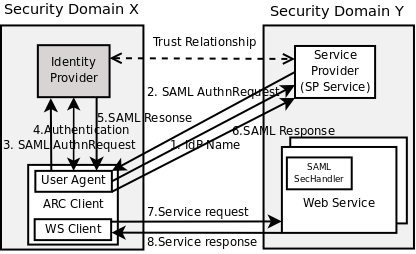
\includegraphics[width=3.2256in,height=1.8472in]{SecurityFrameworkofARC1-img7.png}
\end{center}

\bigskip

{\centering\selectlanguage{english}\itshape\color{black}
Figure \stepcounter{Figure}{\theFigure}.\textbf{ }SAML2.0 SSO profile in
ARC
\par}

{\selectlanguage{english}\color{black}
\ The steps shows in Figure 6 are described as follows:}

\liststyleLi
\begin{enumerate}
\item {\selectlanguage{english}\color{black}
The client uses the user agent interface to launch a HTTP request
including the IdP name (to which the user belongs) to the service side.
The endpoint of the SP (Service Provider) service is the same as that
of the other target services, except the last part of the endpoint is
{\textquotedblleft}saml2sp{\textquotedblright} which is specific for
pointing to the SP Service. Note that we use Identity Provider (IdP)
name here to simplify the IdP discovery process in order to avoid the
IdP discovery process, because we suppose that the user who would
access the target services should better know where is he from
initially.}
\item {\selectlanguage{english}\color{black}
The SP Service searches the metadata (we use the same metadata format as
defined in Shibboleth) and gets the location of the single sign-on
service (hosted in IdP) and also the location of assertion consuming
service (hosted in this SP itself) in order to compose the SAML
{\textless}samlp:AuthnRequest{\textgreater} message. Then SP Service
issues this {\textless}samlp:AuthnRequest{\textgreater} message by
using its own X.509 certificate (note that in the SAML SSO profile,
X.509 certificates are still needed for IdP and SP) and sends back to
user agent.}
\item {\selectlanguage{english}\color{black}
User agent sends the {\textless}samlp:AuthnRequest{\textgreater} message
to the Identity Provider.}
\item {\selectlanguage{english}\color{black}
Identity Provider requires an act of authentication. The authentication
mechanism is outside of the SAML2.0 SSO profile. Shibboleth IdP
implementation chooses some login handlers for authentication. The
current user agent implementation is compatible with the
Username/Password login handler of Shibboleth IdP. Through the HTTP
protocol, the user agent will feed IdP with the username/password which
has been given by the caller of user agent interface.}
\item {\selectlanguage{english}\color{black}
Once the authentication has been succeeded, the IdP issues a SAML
response including an encrypted (encrypted by destination
SP{\textquoteright}s public key) SAML assertion, and then this SAML
response will be delivered by the user agent to the Service Provider.}
\item {\selectlanguage{english}\color{black}
The SP Service verifies and checks the SAML response, decrypts and
stores the SAML assertion into session/connection context. The SAML
assertion includes the {\textless}saml:AuthnStatement{\textgreater} and
{\textless}saml:AttributeStatement{\textgreater}.}
\item {\selectlanguage{english}\color{black}
The WS client launches the Grid/Web Service request via the same
connection as the one which is used by user agent to contact SP
Service.}
\item {\selectlanguage{english}\color{black}
The Grid/Web Service checks the
{\textless}saml:AuthnStatement{\textgreater} from the session context
to see if the session is still valid through the SecHandler called
{\textquotedblleft}SAML SecHandler{\textquotedblright}. If valid,
service handles the service processing and returns the response to WS
client. Note that service requires that WS client is from the same
connection as the one on which user agent contact SP service, in order
to guarantee that the validity of SSO profile result effects the WS
client/Web Service interaction.}
\end{enumerate}
{\selectlanguage{english}\upshape\color{black}
\ \ \ \ The SP service and other functional service(s) are hosted by the
same container, and they use the same X.509 credential. The client
authentication is switched off, so that client doesn{\textquoteright}t
need to use any X.509 credential. Only the trusted certificates (CA
certificates for both SP and IdP) need to be configured for the client
side, so that SP and IdP can authenticate themselves to the client. As
required by the SAML2.0 profile, the SP and IdP should have trust
relationship to each other.}

{\selectlanguage{english}\upshape\color{black}
\ \ \ \ One benefit of the SAML2.0 SSO profile that is worth mentioning
is: the Identity Provider could cache the authentication result through
session management once the user agent has succeeded to authenticate;
then for a short period this authentication result is valid so that the
user agent doesn{\textquoteright}t need to feed IdP with
user{\textquoteright}s username and password the next time (if this
point of time is not out of the scope of valid period) it authenticates
against IdP. So user (or the client on behalf of this user) can travel
across multiple security \ domains with only providing his name and
password once, which is the characteristic of single sign-on.}

{\selectlanguage{english}\upshape\color{black}
\ \ \ \ Since the Shibboleth implementation of SAML is
standard-compliant and widely deployed, the solution implemented in ARC
can easily interoperate with other SAML implementations with minimum
change, and more importantly, this solution can succeed to utilize the
widely deployed SAML implementation for authentication in Grid systems
by avoiding the usage of X.509 certificate.}

{\selectlanguage{english}\upshape\color{black}
\ \ \ \ Moreover, even though the implementation is based on the ARC
middleware, the idea can be adopted by other Grid middlewares if they
only require server authentication instead of mutual authentication.}


\bigskip

\subsection[\ Short-Lived Credential
Service]{\foreignlanguage{english}{\ }Short-Lived Credential Service}
{\selectlanguage{english}\color{black}
\ \ \ \ However, most of the widely used Grid middlewares are based on
GSI while GSI requires mutual authentication. Also for Web Service
based Grid solution, we cannot prevent service side from requiring
client X.509 certificate. Based on the solution described in Section 9,
a short lived credential service (SLCS) is implemented by which user
can get a short-lived X.509 certificate without being bothered to
contact any registration authority (RA) or certificate authority (CA).}

{\selectlanguage{english}\color{black}
\ \ \ \ The SLCS service is also a Web Service (standard Web Service
implemented by using ARC service interface), and the SLCS client is a
specific command-line interface (CLI) which includes the user agent and
WS client. The whole process of SLCS invocation is showed in Figure 7
(from step 1 to step 8), which is the same as in Figure 6, except that
step 7 and step 8 are invoked for the SLCS certificate request and
response.}



\begin{center}
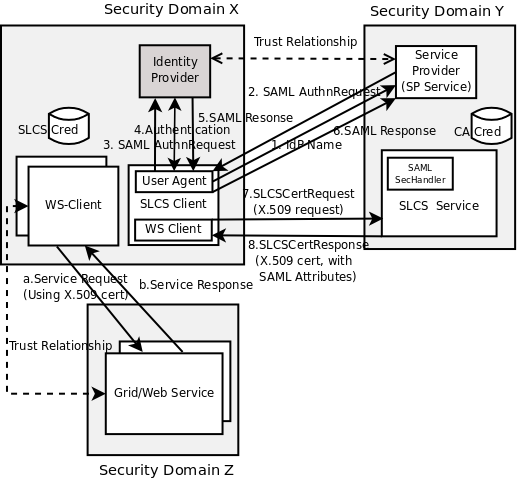
\includegraphics[width=3.7689in,height=3.2055in]{SecurityFrameworkofARC1-img8.png}
\end{center}
{\centering\selectlanguage{english}\itshape\color{black}
Figure \stepcounter{Figure}{\theFigure}.Short lived credential service
\par}


\bigskip

{\selectlanguage{english}\color{black}
\ \ \ \ SLCS service is supposed to run together with SP service for
achieving the SAML2 SSO profile. A typical configuration for SLCS
service is as follows:}

\begin{center}
\tablehead{}\begin{supertabular}{|m{5.6886597in}|}
\hline
{\selectlanguage{english}\itshape\color{black}
\ \ \ \ {\textless}/Chain{\textgreater}}

{\selectlanguage{english}\itshape\color{black}
\ \ \ \ \ \ \ \ {\textless}Component
name={\textquotedbl}tcp.service{\textquotedbl}
id={\textquotedbl}tcp{\textquotedbl}{\textgreater}}

{\selectlanguage{english}\itshape\color{black}
\ \ \ \ \ \ \ \ \ \ \ \ {\textless}next
id={\textquotedbl}tls{\textquotedbl}/{\textgreater}}

{\selectlanguage{english}\itshape\color{black}
\ \ \ \ \ \ \ \ \ \ \ \ {\textless}tcp:Listen{\textgreater}{\textless}tcp:Port{\textgreater}60000{\textless}/tcp:Port{\textgreater}{\textless}/tcp:Listen{\textgreater}}

{\selectlanguage{english}\itshape\color{black}
\ \ \ \ \ \ \ \ {\textless}/Component{\textgreater}}

{\selectlanguage{english}\itshape\color{black}
\ \ \ \ \ \ \ \ {\textless}Component
name={\textquotedbl}tls.service{\textquotedbl}
id={\textquotedbl}tls{\textquotedbl}{\textgreater}}

{\selectlanguage{english}\itshape\color{black}
\ \ \ \ \ \ \ \ \ \ \ \ {\textless}next
id={\textquotedbl}http{\textquotedbl}/{\textgreater}}

{\selectlanguage{english}\itshape\color{black}
\ \ \ \ \ \ \ \ \ \ \ \ {\textless}tls:KeyPath{\textgreater}./testkey-nopass.pem{\textless}/tls:KeyPath{\textgreater}}

{\selectlanguage{english}\itshape\color{black}
\ \ \ \ \ \ \ \ \ \ \ \ {\textless}tls:CertificatePath{\textgreater}./testcert.pem{\textless}/tls:CertificatePath{\textgreater}}

{\selectlanguage{english}\itshape\color{black}
\ \ \ \ \ \ \ \ \ \ \ \ {\textless}!-{}-tls:CACertificatePath{\textgreater}./cacert.pem{\textless}/tls:CACertificatePath-{}-{\textgreater}}

{\selectlanguage{english}\itshape\color{black}
\ \ \ \ \ \ \ \ \ \ \ \ {\textless}tls:ClientAuthn{\textgreater}false{\textless}/tls:ClientAuthn{\textgreater}}

{\selectlanguage{english}\itshape\color{black}
\ \ \ \ \ \ \ \ {\textless}/Component{\textgreater}}

{\selectlanguage{english}\itshape\color{black}
\ \ \ \ \ \ \ \ {\textless}Component
name={\textquotedbl}http.service{\textquotedbl}
id={\textquotedbl}http{\textquotedbl}{\textgreater}}

{\selectlanguage{english}\itshape\color{black}
\ \ \ \ \ \ \ \ \ \ \ \ {\textless}next
id={\textquotedbl}plexer{\textquotedbl}{\textgreater}POST{\textless}/next{\textgreater}}

{\selectlanguage{english}\itshape\color{black}
\ \ \ \ \ \ \ \ {\textless}/Component{\textgreater}}

{\selectlanguage{english}\itshape\color{black}
\ \ \ \ \ \ \ \ {\textless}Plexer
name={\textquotedbl}plexer.service{\textquotedbl}
id={\textquotedbl}plexer{\textquotedbl}{\textgreater}}

{\selectlanguage{english}\itshape\color{black}
\ \ \ \ \ \ \ \ \ \ \ \ {\textless}next
id={\textquotedbl}samlsp{\textquotedbl}{\textgreater}/saml2sp{\textless}/next{\textgreater}}

{\selectlanguage{english}\itshape\color{black}
\ \ \ \ \ \ \ \ \ \ \ \ {\textless}next
id={\textquotedbl}soap{\textquotedbl}{\textgreater}/slcs{\textless}/next{\textgreater}}

{\selectlanguage{english}\itshape\color{black}
\ \ \ \ \ \ \ \ {\textless}/Plexer{\textgreater}}

{\selectlanguage{english}\itshape\color{black}
\ \ \ \ \ \ \ \ {\textless}Component
name={\textquotedbl}soap.service{\textquotedbl}
id={\textquotedbl}soap{\textquotedbl}{\textgreater}}

{\selectlanguage{english}\itshape\color{black}
\ \ \ \ \ \ \ \ \ \ \ \ {\textless}next
id={\textquotedbl}slcs{\textquotedbl}/{\textgreater}}

{\selectlanguage{english}\itshape\color{black}
\ \ \ \ \ \ \ \ \ \ \ \ {\textless}SecHandler
name={\textquotedbl}saml2ssoserviceprovider.handler{\textquotedbl}
id={\textquotedbl}saml2ssosp{\textquotedbl}
event={\textquotedbl}incoming{\textquotedbl}/{\textgreater}}

{\selectlanguage{english}\itshape\color{black}
\ \ \ \ \ \ \ \ {\textless}/Component{\textgreater}}

{\selectlanguage{english}\itshape\color{black}
\ \ \ \ \ \ \ \ {\textless}Service
name={\textquotesingle}saml.sp{\textquotesingle}
id={\textquotesingle}samlsp{\textquotesingle}{\textgreater}}

{\selectlanguage{english}\itshape\color{black}
\ \ \ \ \ \ \ \ \ \ \ \ {\textless}MetaDataLocation{\textgreater}./test\_metadata.xml{\textless}/MetaDataLocation{\textgreater}}

{\selectlanguage{english}\itshape\color{black}
\ \ \ \ \ \ \ \ \ \ \ \ {\textless}ServiceProviderName{\textgreater}https://squark.uio.no/shibboleth-sp{\textless}/ServiceProviderName{\textgreater}}

{\selectlanguage{english}\itshape\color{black}
\ \ \ \ \ \ \ \ {\textless}/Service{\textgreater}}

{\selectlanguage{english}\itshape\color{black}
\ \ \ \ \ \ \ \ {\textless}Service
name={\textquotedbl}slcs.service{\textquotedbl}
id={\textquotedbl}slcs{\textquotedbl}{\textgreater}}

{\selectlanguage{english}\itshape\color{black}
\ \ \ \ \ \ \ \ \ \ \ \ {\textless}next
id={\textquotedbl}slcs{\textquotedbl}/{\textgreater}}

{\selectlanguage{english}\itshape\color{black}
\ \ \ \ \ \ \ \ \ \ \ \ {\textless}slcs:CACertificate{\textgreater}./CAcert.pem{\textless}/slcs:CACertificate{\textgreater}}

{\selectlanguage{english}\itshape\color{black}
\ \ \ \ \ \ \ \ \ \ \ \ {\textless}slcs:CAKey{\textgreater}./CAkey.pem{\textless}/slcs:CAKey{\textgreater}}

{\selectlanguage{english}\itshape\color{black}
\ \ \ \ \ \ \ \ \ \ \ \ {\textless}slcs:CASerial{\textgreater}./CAserial{\textless}/slcs:CASerial{\textgreater}}

{\selectlanguage{english}\itshape\color{black}
\ \ \ \ \ \ \ \ {\textless}/Service{\textgreater}}

\selectlanguage{english}\itshape\color{black}
\ \ \ \ {\textless}/Chain{\textgreater}\\\hline
\end{supertabular}
\end{center}
{\selectlanguage{english}\color{black}
\ \ \ \ As shown in the above table, a plexer dispatches the message
flow (outgoing from \textit{http.service}) into two SP service
(\textit{saml.sp}) and SOAP service (\textit{soap.service}). Since the
client authentication is switched off, it is not necessary to configure
{\textless}\textit{CACertificatePath}{\textgreater} or
{\textless}\textit{CACertificateDir}{\textgreater} for TLS MCC.}

{\selectlanguage{english}\color{black}
\ \ \ \ SP service needs to be configured with
{\textless}\textit{MetaDataLocation}{\textgreater} and
{\textless}\textit{ServiceProviderName}{\textgreater}. }

{\selectlanguage{english}\color{black}
\ \ \ \ SLCS service needs to be configured with
{\textless}\textit{CACertificate}{\textgreater}
{\textless}\textit{CAKey}{\textgreater} and
{\textless}\textit{Caserial}{\textgreater}.}

{\selectlanguage{english}\color{black}
\ \ \ \ SLCS client generates \ a X.509 certificate \ request, launches
a Web Service request which includes the certificate request; SLCS
service then gets the certificate request, composes a distinguished
name (DN), issues a certificate (short lived, 12 hours by default) with
the SAML attribute (from the SAML2.0 SSO profile) as the X.509
certificate extension, and puts the certificate in to the Web Service
response; SLCS client get the response and stores the X.509 certificate
into local repository.}

{\selectlanguage{english}\color{black}
The CLI for the SLCS client is like this:}

{\selectlanguage{english}\ttfamily\color{black}
\$ ./arcslcs -S https://127.0.0.1:60000/slcs -I
https://idp.testshib.org/idp/shibboleth -U myself -P myself}

{\selectlanguage{english}\color{black}
\ \ \ \ Since the lifetime of the short lived credential is normally
short, it is not a must to protect the private key by a pass phrase. As
illustrated in steps (a) and (b) in Figure 7, if the private key is not
protected through the Web Service client, the user can use the X.509
certificate to access Grid Service or Web Service from any kind of
middleware. If the private key is protected, she can use the X.509
certificate to generate a proxy certificate (by using a command-line
interface utility such as grid-proxy-init , voms-proxy-init, or
arcproxy ), and then use the proxy certificate to access a Grid/Web
Service.}

{\selectlanguage{english}\color{black}
\ \ \ \ It is worth mentioning that since the ARC middleware can support
GSI communication by configuring the GSI MCC, together with the X.509
certificate, the Web Service client developed with the ARC Web Service
client interface can interoperate with Grid Service that requires GSI
communication.}

{\selectlanguage{english}\color{black}
\ \ \ \ It should be noticed that the process of composing the
distinguished name (DN) for the certificate is a critical issue for the
SLCS service. Since the Shibboleth Identity Provider uses the eduPerson
schema for the definition of {\textless}saml:Attribute{\textgreater} in
{\textless}saml:AttributeStatement{\textgreater}, we pick the
relatively distinguishable attribute
{\textquotedblleft}eduPersonPrincipalName{\textquotedblright} for the
DN. A typical eduPersonPrincipalName value could be alice@example.org,
then the DN is
{\textquotedblleft}/O=knowarc/OU=example.org/CN=alice{\textquotedblright}.}

{\selectlanguage{english}\color{black}
\ \ \ \ The obvious benefit of the SLCS service is that: If a user
passes the authentication to her home Identity Provider, she can get
the X.509 credential anywhere simply by running the SLCS client command
together with providing her username and password to this home IdP, and
then access the Grid system conveniently. Thanks to the single sign-on
characteristic of SAML2.0 SSO profile, this user
doesn{\textquoteright}t not need to input her username and password in
a valid period after the first time she succeeds to authenticate
against her home IdP by running the SLCS client command on the same
node, even if this SLCS client command is supposed to run against a few
SLCS services to get a few SLCS credentials.}


\bigskip


\bigskip

\subsection[\ X.509 Credential Delegation
Service]{\selectlanguage{english}\scshape\color{black} \ X.509
Credential Delegation Service}

\bigskip

\clearpage{\centering\selectlanguage{english}\bfseries\scshape\color{black}
References
\par}

{\selectlanguage{english}\color{black}
\stepcounter{Bibitem}{\theBibitem}. RFC3820- Internet X.509 Public Key
Infrastracture (PKI) Proxy, \url{http://rfc.net/rfc3820.html}}

{\selectlanguage{english}\color{black}
\stepcounter{Bibitem}{\theBibitem}. D1.2-2 The ARC container (first
prototype),
\url{http://www.knowarc.eu/documents/Knowarc_D1.2-2_07.pdf}}

{\selectlanguage{english}\color{black}
\textstyleInternetlink{\textcolor{black}{\stepcounter{Bibitem}{\theBibitem}}}\textstyleInternetlink{\textcolor{black}{.}}\textstyleInternetlink{\foreignlanguage{english}{\textcolor{black}{Web
Service Security Username Token Profile 1.1.
}}}\url{http://www.oasis-open.org/committees/download.php/16782/wss-v1.1-spec-os-UsernameTokenProfile.pdf}}

{\selectlanguage{english}\color{black}
\stepcounter{Bibitem}{\theBibitem}. OGSA{\textregistered} Basic
Execution Service Version 1.0,
\ \url{http://www.ogf.org/documents/GFD.108.pdf} }

{\selectlanguage{english}\color{black}
\textstyleInternetlink{\textcolor{black}{\stepcounter{Bibitem}{\theBibitem}}}\textstyleInternetlink{\textcolor{black}{.
OASIS Web Services Security (WSS) TC.
}}\url{http://www.oasis-open.org/committees/tc_home.php?wg_abbrev=wss}}
\end{document}
